% Класс документа пока не окончательный, сильно сомневаюсь, что article 		
\documentclass[a4paper,12pt]{extarticle} 
% Подключаем шрифты,кодировки,русские переносы
\usepackage{cmap}
% подключается пакет, позволяющий улучшить вид пдф документа(как я понял)
\usepackage[utf8x]{inputenc}
% подключаем кодировку шрифтов для вносимых файлов
\usepackage[T2A]{fontenc}
% подключаем кодировку внутреннних шрифтов
\usepackage[main=russian,english]{babel}
% подключаем перенос и распознование слов, русский в приоритете
\usepackage{indentfirst}
% Отступ в начале абзаца
% \usepackage[unicode=true,pdfusetitle,
 	% bookmarks=true,bookmarksnumbered=false,bookmarksopen=true,
 	% breaklinks=false,pdfborder={0 0 0},pdfborderstyle={},backref=slide,colorlinks=false]
 	% {hyperref}
 % Надо разобраться с опциями, копирнул из пред.файла, который еще был написан в lyx
\usepackage{subfig}
% попытка загрузить minipage
\usepackage{
	amssymb,
	amsfonts,
	amsmath,
}
\usepackage{nicefrac}
% Пакеты американского математ. сообщества, красивый вид формул и текста внутри, а также дробный вид формул
\usepackage{esdiff}
% Пакет для производных
\usepackage{
	wrapfig,
	graphicx,
	caption,
	% subcaption,
	tikz,
}
\captionsetup{format=plain,labelsep=period}
% Обтекаемые объекты, рисунки, подписи без двоеточий и прочее
\usepackage{
	pgfplotstable,
	pgfplots,
	booktabs,
	colortbl,
	array,
	% float
}
\pgfplotsset{compat=newest}
% таблицы, графики
\usepackage[final]{pdfpages}
% Для вставки pdf файлов
\usepackage{geometry}
\usepackage{fancyhdr}
% границы, контитулы, и прочее


\geometry
	{
	left=1.5cm,
	right=1.5cm,
	bottom=2cm,
	top=2cm,
	}
% границы документа

\usepackage{setspace}
% убирает гигантские размеры оглавления
\linespread{1.3}
% междустрочный интервал

\pagestyle{fancy}
\fancyhead{}
% пустая шапка контитула
\fancyhead[R]{\authors}
% На правой стороне страницы авторы и науч.рук.
\fancyhead[L]{\labname}
 % Слева название лабы
\fancyfoot{}
\fancyfoot[C]{\thepage}
% номер страницы снизу по середине
\renewcommand{\contentsname}{Оглавление}
% переводим на русский язык оглавление
\usepackage{secdot}
\sectiondot{subsection}
% Ставит злосчастные точки в главах, ибо не по госту
% Преамбула почти слизана у Федора Сарафанова https://github.com/FedorSarafanov/RLC/blob/master/text/diss.tex

\usepackage{xcolor}
\usepackage{float}
\usepackage{hyperref}
\usepackage{tikz}
\usepackage{pgfplots}
\hypersetup{unicode=true}
\definecolor{linkcolor}{HTML}{799B03} % цвет ссылок
\definecolor{urlcolor}{HTML}{799B03} % цвет гиперссылок

\hypersetup{pdfstartview=FitH,  linkcolor=linkcolor,urlcolor=urlcolor, colorlinks=true}
\begin{document}
	\sloppy
	\def\authors{Есюнин М.В., Есюнин Д.В.}
	\def\labnum{6}
	\def\labname{Исследование нелиненых преобразований сигналов}
	\def\sciadviser{Орлов И.Я.}
	% \renewcommand{\contentsname}{Оглавление}
	% \renewcommand{\figurename}{Рис.}
	\renewcommand{\vec}{\mathbf}
	\renewcommand{\phi}{\varphi}
	\renewcommand{\kappa}{\varkappa}
	% нормальный вид вектора, фи и каппа
	\renewcommand{\Re}{\operatorname{Re}}
	\renewcommand{\Im}{\operatorname{Im}}
	% меняем номрмальное начертание Re and Im
	\begin{titlepage}

\begin{center}

	\textsc{Нижегородский государственный университет имени Н.\,И. Лобачевского}
	\vskip 4pt \hrule \vskip 8pt
	\textsc{Радиофизический факультет}

	\vfill

	{\Large Отчет по лабораторной работе №\labnum \vskip 20pt\bfseries \labname}

\end{center}

\vfill

\begin{flushright}
	{Работу выполнили студенты\\ \authors\\ 430 группы\\ \vskip 14pt Преподаватель:\\ \sciadviser}
\end{flushright}

\vfill

\begin{center}
	Нижний Новгород, \the\year
\end{center}

\end{titlepage}
	\begin{spacing}{1.2}
		\tableofcontents
	\end{spacing}
	
	\newpage
\section{Цель работы}
Изучение основных процессов происходящих при прохождении сигналов через радиотехнические цепи с нелинейным элементом, экспериментальное исследование полупроводникового преобразователя частоты и амплитудного диодного детектора.
\section{Назначение устройств}
Исследуемые в лабораторной работе устройства используются для нелинейного преобразования сигналов. Преобразователь частоты -- для перемещения спектра сигнала по шкале частот без изменения характера сигнала, т.е. соотношений между компонентами спектра. Например, для модулированных колебаний это означает изменение (повышение или понижение) несущей частоты с сохранением вида модуляции и закона изменения модулированного параметра. Амплитудный детектор -- для преобразования модулированного колебания в низкочастотное колебание, соответствующее модулирующему сигналу.

Основные радиотехнические преобразования сигналов осуществляются с помощью нелинейных цепей. Поэтому свойства нелинейных элементов и цепей являются фундаментом для теории большинства радиотехнических устройств.

Нелинейным называются цепи, описываемые нелинейным дифференциальными уравнениями вида \eqref{eq:1},
\begin{equation}
a_0\frac{d^ny}{dt^n}+a_1\frac{d^{n-1}y}{dt^{n-1}}+\cdots+a_ny=b_0\frac{d^mx}{dt^m}+b_1\frac{d^{m-1}x}{dt^{m-1}}+\cdots+b_mx
\label{eq:1}
\end{equation}
в которых хотя бы один из коэффициентов $a_i$ является функцией $y$ или ее производных, либо один из коэффициентов $b_i$ -- функцией $x$ или её производных:
\begin{equation*}
a_i=a_i(y,\frac{dy}{dt},\cdots),\;b_i=b_i(y,\frac{dx}{dt},\cdots)
\end{equation*}

Уравнение электрической цепи оказывается нелинейным в том случае, когда в схеме используются какие-либо нелинейные элементы, т.е элементы параметры, которых зависят от тока или напряжения. Нелинейными являются все электронные и полупроводниковые приборы. Особенности этих приборов определяются вольт-амперными характеристиками, т.е. зависимостями токов от приложенных напряжений. 
\section{Аппроксимация вольт-амперных характеристик}
Математическое описание работы радиотехнической цепи начинается с составления уравнений, связывающих токи и напряжения в различных частях ее, в том числе и в нелинейных элементах. Для нелинейных элементов обычно известна графическая зависимость тока от напряжения (из справочника или эксперимента). Поэтому в радиотехнике широкое распространение получили способы представления вольт-амперных характеристик простыми функциями, приближенно отображающими истинные характеристики. Замена истинной характеристики приближенно представляющей ее функцией называется аппроксимацией характеристики.

Выбор аппроксимирующей функции зависит от вида нелинейности, а также от режима работы нелинейного элемента.
\subsection{Полиномиальная аппроксимация}
Одним из наиболее распространенных способов аппроксимации является аппроксимация степенным полиномом. Полиномиальная аппроксимация заключается в представлении вольт-амперной характеристики $i=f(u)$ полиномом $n-$й степени. Такой способ аппроксимации является удобным для объяснения принципа действия многих нелинейных устройств.

Запишем аппроксимирующий степенной полином в форме:
\begin{equation}
i(v_0+u)=i(v_0)+a_1u+a_2u^2+\cdots+a_nu^n
\label{eq:2}
\end{equation}
где $v_0$ - напряжение, определяющее исходное положение рабочей точки на характеристике нелинейного элемента (в отсутствие сигнала) , $u$ -- подаваемое на нелинейный элемент напряжение сигнала. Коэффициенты $a_1,\;a_2,\;a_3\cdots$ определяются выражениями
\begin{equation}
a_1=\left(\frac{di}{du}\right)_{u=v_0},\;a_2=\frac{1}{2}\left(\frac{d^2i}{du^2}\right)_{u=v_0},\;a_2=\frac{1}{3!}\left(\frac{d^3i}{du^3}\right)_{u=v_0}
\label{eq:3}
\end{equation}
Нетрудно видеть, что $a_1$ представляет крутизну $S$ вольт-амперной характеристики $S=(di/du)_{u=v_0}$ в рабочей точке $u=v_0$,
$a_2$ -- первую производную крутизны (с коэффициентом 1/2!),
$a_3$ -- вторую производную крутизны (с коэффициентом 1/3!) и т.д. При заданной форме вольт-амперной характеристики, величины коэффициентов $a_1,\;a_2,\;a_3$ существенно зависят от положения начальной рабочей точки на характеристике.
\begin{wrapfigure}[12]{l}{0.5\linewidth}
	\centering
	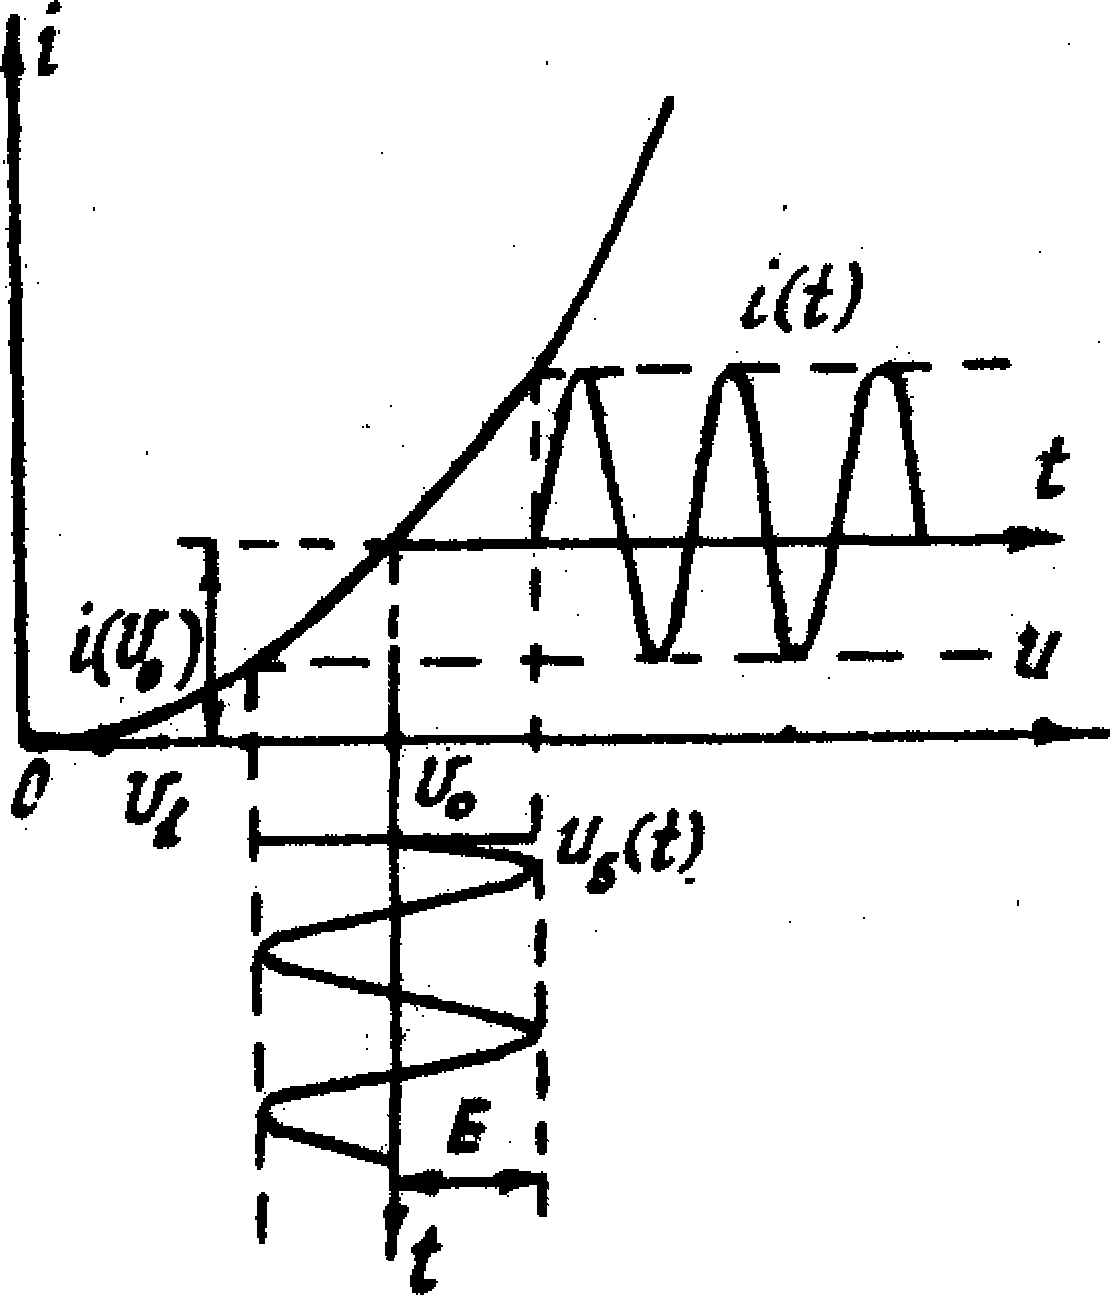
\includegraphics[width=0.6\linewidth]{picture/pic1}
	\caption{}
	\label{pic:1}
\end{wrapfigure}

Например, рабочая точка расположена на начальном участке вольт-амперной характеристики, имеющем вид квадратичной параболы рис.~\ref{pic:1} и подводимое к нелинейному элементу напряжение сигнала $u_s$, накладываясь на постоянное напряжение $E_0=v_0$ не выходит за точку $v_1$, т.е. за начало характеристики.
Выражение \eqref{eq:2} в данном случае можно записать в вине полинома второй степени $i(v_0+u_s)=i(v_0)+a_1u_s+a_2u_s^2$ 

Коэффициент $a_2$ определяется из условия, что при $u_s=v_1-v_0$, ток $i=0$, откуда вытекает уравнение
\begin{equation*}
i(v_0)+S(v_1-v_0)+a_2(v_1-v_0)^2=0
\end{equation*}
определяющее
\begin{equation*}
a_2=-\frac{i(v_0)+S(v_1-v_0)}{(v_1-v_0)^2}
\end{equation*}
\subsection{Кусочно-линейная аппроксимация}
Кусочно-линейная аппроксимация заключается в замене реальной плавно меняющейся зависимости $i=f(u)$ приближенной, состоящей из отрезков прямых линий, выбираемых, касательными к реальной характеристике в нескольких точках.

Например, если рабочая точка $v_0$ находится на нижнем сгибе характеристики и изменение подводимого напряжения настолько велико, что используется участок $ab$ на оси абсцисс, то характеристика аппроксимируется выражениями
\begin{equation*}
i = \begin{cases} 
0, & \text{при $u\leq v_1$;} \\ 
s(u-v_1), & \text{при $u\geq v_1$.} 
\end{cases}
\end{equation*}
\begin{figure}[h!]
	\begin{minipage}{0.49\linewidth}
		\centering
		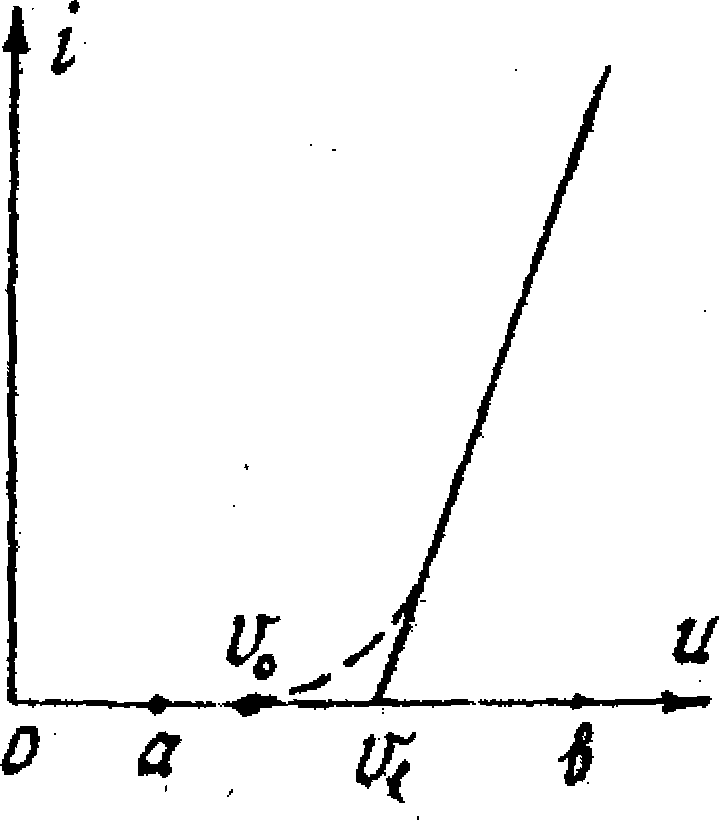
\includegraphics[width=0.5\linewidth]{picture/pic21}
	\end{minipage}
	\begin{minipage}{0.49\linewidth}
		\centering
		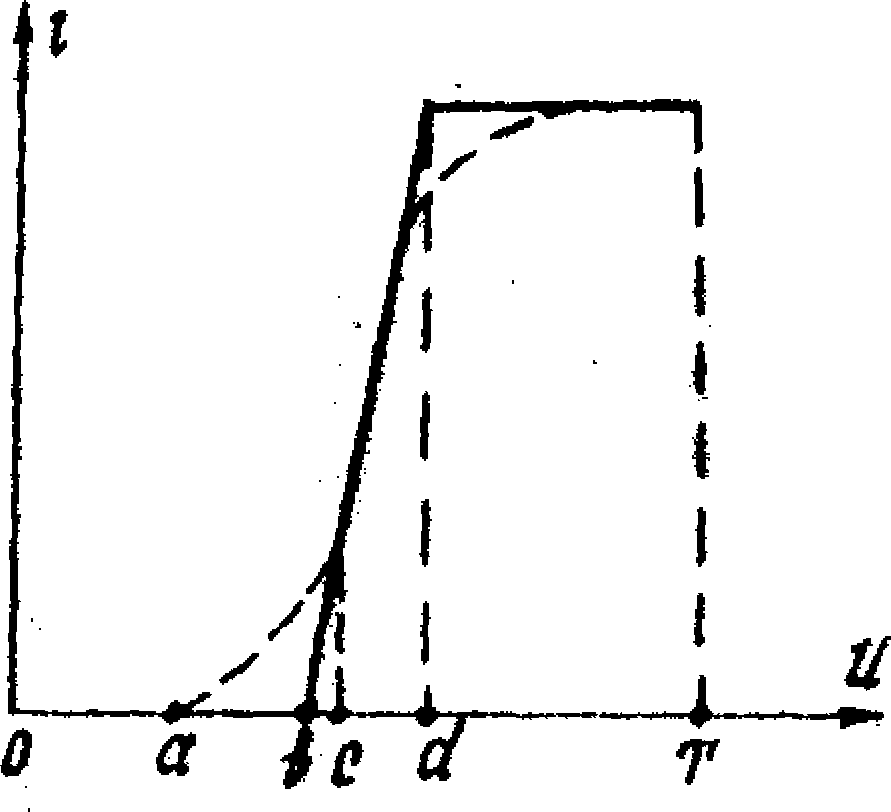
\includegraphics[width=0.6\linewidth]{picture/pic22}
	\end{minipage}
\caption{}
\label{pic:2}
\end{figure}
На рис.~\ref{pic:2} показана такая аппроксимация, содержащая два линейных участка. Данная аппроксимация широко используется при рассмотрений воздействия сигналов большой амплитуды. Если же амплитуда входного сигнала невелика, наблюдается значительное различие в результатах расчета по действительной и аппроксимированной характеристикам, т.е. такая аппроксимация непригодна.
\section{Метод определения спектра сигнала на выходе нелинейной цепи}
При рассмотрении функциональных преобразований сигналов возникает задача определения спектра колебаний на выходе нелинейной цепи. Одной из важнейших особенностей нелинейных цепей является то, что в них не выполняется принцип суперпозиции. Поэтому спектральный метод широко используемый в теории линейных цепей, непригоден для анализа нелинейных цепей.

Задача заключается в следующем: на вход безынерционного нелинейного элемента, с характеристикой аппроксимируемой зависимостью
\begin{equation}
i=f(u)
\label{eq:4}
\end{equation}
действует гармоническое
\begin{equation}
u=l_s(t)=E_1\cos(\omega_1t+\phi)
\label{eq:5}
\end{equation}
или полигармоническое колебание
\begin{equation}
u=l_s(t)=\sum_{k=1}^{n}E_k\cos(\omega_kt+\phi)
\label{eq:6}
\end{equation}
Требуется определить спектр отклика, т.е. спектр тока $i$ \eqref{eq:4}.
Классический метод решения заключается в подстановке выражений \eqref{eq:5}, \eqref{eq:6} в правую часть \eqref{eq:4} с последующим определением спектральных компонент путем использования аппарата рядов Фурье в случае гармонического воздействия или кратных рядов Фурье в случае полигармонического воздействия. Однако такой метод оказывается очень трудоемким. Поэтому на практике применяются специальные методы, каждый из которых связан с определенными способами аппроксимации нелинейной зависимости \eqref{eq:4} и характером воздействующего сигнала.

Наибольшее распространение имеют методы, основанные на использовании: 1) тригонометрических Формул кратного аргумента и 2) угла отсечки.
\section{Метод, основанный на использовании тригонометрических формул кратного аргумента}
Этот метод является основным при использовании полиномиальной аппроксимации и особенно удобен для выяснения принципа действия и основных особенностей таких устройств, как модуляторы, детекторы, преобразователи частоты и т.п. Рассмотрим воздействие на нелинейный элемент, характеристика которого аппроксимирована полиномом $n$-ой степени
\begin{equation}
i=a_0+a_1u+\cdots+a_nu^n
\label{eq:7}
\end{equation}
гармонического колебания \eqref{eq:5}. Подставляя \eqref{eq:5} в \eqref{eq:7} получим. 
\begin{equation}
i=a_0+a_1E_1\cos(\omega_1t+\phi)+\cdots+a_nuE_1^n\cos^n(\omega_1t+\phi)
\label{eq:8}
\end{equation}

Для представления правой части \eqref{eq:8} в виде суммы синусоидальных компонент воспользуемся известными тригонометрическими формулами, позволяющими заменить степени косинусов (или синусов) через тригонометрические функции кратных аргументов. Выполнив тригонометрические преобразования, выражение \eqref{eq:8} приводим к виду
\begin{equation}
i=\gamma_0+\gamma_1\cos(\omega_1t+\phi)+\gamma_2\cos(2\omega_1t+\phi)+\cdots+
\gamma_n\cos(n\omega_1t+\phi)
\label{eq:9}
\end{equation}
где $\displaystyle \gamma_0=a_0+\frac{1}{2}a_2E_1^2+\frac{3}{8}a_4E_1^4+\cdots$постоянная составляющая тока нелинейного элемента, 
$\gamma_1=a_1E_1+\frac{3}{4}a_3E_1^3+\frac{5}{8}a_5E_1^5+\cdots$ -- амплитуда первой гармоники.

\noindent $\gamma_2=\frac{1}{1}a_2E_1^2+\frac{1}{2}a_4E_1^4+\cdots$ -- амплитуда второй гармоники.

\noindent $\gamma_3=\frac{1}{4}a_3E_1^3+\frac{5}{16}a_5E_1^5+\cdots$ - амплитуда третьей гармоники.

\noindent $\gamma_n$ -- амплитуда $n$-ой гармоники.

\begin{wrapfigure}[8]{l}{0.5\linewidth}
	\centering
	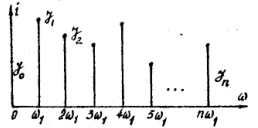
\includegraphics[]{picture/pic3.jpg}
	\caption{}
	\label{pic:3}
\end{wrapfigure}

На рис.~\ref{pic:3} построен спектр выходного тока. Из сравнения \eqref{eq:9} c \eqref{eq:5} следует:

	1. Спектр тока нелинейного элемента при воздействии на него гармонического сигнала оказывается линейчатым, содержащим составляющие с частотами, кратными частоте входного сигнала. Наивысший номер составляющей спектра получаемой пои расчетах равен степени используемого аппроксимирующего полинома. Поэтому если для какого-то применения нелинейного элемента необходимо знать $n$--ю гармонику, вольт-амперная характеристика его при расчетах должна быть аппроксимирована полиномом не ниже $n$--го порядка.
	2. Постоянная составляющая и амплитуды четных гармоник определяются четными степенями напряжения в полиноме \eqref{eq:7}, а нечетных гармоник -- только нечетными.
	3. Текущая фаза $\psi_k$--ой гармоники с частотой $\omega_k=k\omega_1$ в $k$ раз больше значения текущей фазы воздействующего сигнала
\begin{equation*}
\psi_k=\omega_k+\phi_k=k(\omega_1+\phi)
\end{equation*}
Начальный фазы связаны соотношением $\phi_k=k\phi$

Рассмотрим воздействие на нелинейный элемент бигармонического колебания
\begin{equation}
l_s(t)=E_1\cos\omega_1t+E_2\cos\omega_2t.
\label{eq:10}
\end{equation}
Ограничимся рассмотрением режима когда достаточно учитывать только линейный и квадратичный члены в полиноме \eqref{eq:2}. 
Подстановка \eqref{eq:10} в \eqref{eq:2} приводит к следующим результатам:
-для линейного члена ряда 
\begin{equation}
l_s(t)=E_1\cos\omega_1t+E_2\cos\omega_2t;
\label{eq:11}
\end{equation}
-для квадратичного члена ряда 
\begin{equation}
\begin{split}
a_2l_s^2(t)=a_2(E_1\cos\omega_1t+E_2\cos\omega_2t)^2 = \\
\frac{1}{2}a_2(E_1^2+E_2^2)+\frac{1}{2}a_2E_1^2\cos2\omega_1t+\frac{1}{2}a_2E_2^2\cos2\omega_2t+\\
a_2E_1E_2[\cos(\omega_1+\omega_2)t+\cos(\omega_1-\omega_2)t]
\label{eq:12}
\end{split}
\end{equation}
Первое слагаемое, не зависящее от времени, определяет приращение постоянного тока. Слагаемые с частотами $2\omega_1$ и $2\omega_2$ представляют собой вторые гармоники от соответствующих компонентов входного сигнала. Слагаемые с частотами $\omega_1+\omega_2$ и $\omega_1-\omega_2$ представляют собой колебания комбинационных частот.

В более общем случае, если в качестве аппроксимирующего полинома взять полином $k^u$ -- степени, при бигармоническом воздействии на нелинейное устройство, в спектре колебания на выходе нелинейного элемента, могут присутствовать следующие частоты:
$\omega=0$ -- постоянная составляющая; $\omega=n\omega_1$, $n=1,2,\ldots k$ -- гармоники частоты $\omega_1$; $\omega=n\omega_2$, $n=1,2,\ldots k$ -- гармоники частоты $\omega_2$; $\omega=|n\omega_1\pm m\omega_2|$, $n=1,2,\ldots k$, $m=1,2,\ldots k$ -- комбинационные частоты (при условии $n+m\leq k$).

Спектрограмма колебания на входе и выходе нелинейного элемента, описываемого полиномом второй степени ( $k=2$) изображена на рис.\ref{pic:4}.
\begin{figure}[h!]
	\centering
	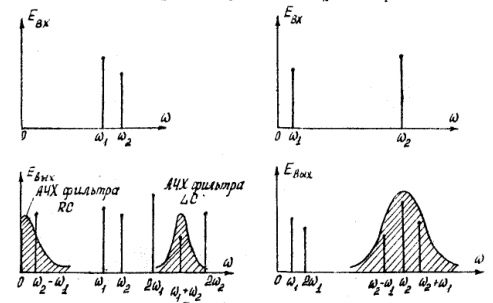
\includegraphics[width=0.8\linewidth]{picture/pic4.jpg}
	\caption{}
	\label{pic:4}
\end{figure}

Из рисунка видно, что взаимодействие двух гармонических колебаний с неодинаковыми частотами в нелинейном устройстве второй степени приводит к возникновению разностной $|\omega_1-\omega_2|$ и суммарной $\omega_1+\omega_2$ частот (помимо гармоник $2\omega_1$	и $2\omega_2$)
Для практического использования этих новых частот достаточно включить последовательно с нелинейным элементом линейную цепь (фильтр), выделяющий полезную составляющую спектра.

Свойство квадратичного нелинейного элемента, позволяющее получить комбинационные частоты, широко применяется в радиотехнике для сдвига частоты сигнала.

И в случае $\omega_1\ll\omega_2$, когда комбинационные частоты располагаются близи частоты $\omega_2$ и  все три частоты: $\omega_1;\;\omega_2+\omega_1$ и $\omega_2-\omega_1$ могут быть выделены одним общим фильтром (см.рис.\ref{pic:4}), можно получить спектр, соответствующий амплитудной модуляции колебания частоты $\omega_2$ относительно низкой частотой $\omega_1$. При нелинейности более высокого порядка ($k>2$) можно осуществить выделение любой из частот вида $\omega=|n\omega_1\pm m\omega_2|,\;n+m\leq k$
При более сложном составе входного спектра, содержащем частоты $\omega_1,\;\omega_2,\;\omega_3,\;\omega_4,\ldots$, на выходе нелинейного элемента возникают частоты $n\omega_1,\;n\omega_2,\;n\omega_3,\;n\omega_4,\ldots$ и комбинационные
частоты	$n\omega_i\pm m\omega_k$, где $n$ и $m$ любые целые числа, а $\omega_i$ и $\omega_k$ -- любая из пар частот входного спектра.
\section{Метод угла отсечки}
Рассмотрим теперь работу нелинейного элемента в случае кусочно-линейной аппроксимации вольт-амперной характеристики рис.~\ref{pic:5}.
\begin{figure}[h!]
	\centering
	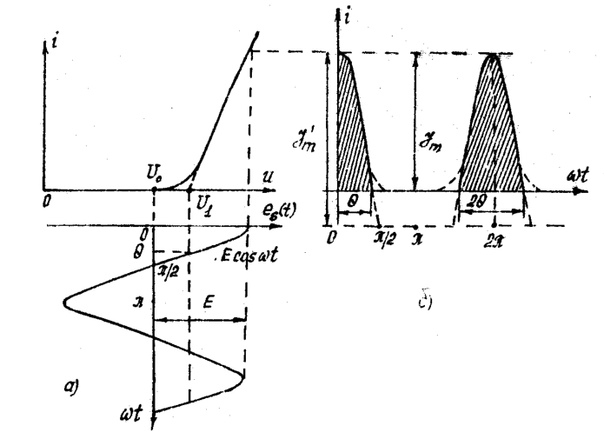
\includegraphics[width=0.7\linewidth]{picture/pic5.jpg}
	\caption{}
	\label{pic:5}
\end{figure}
При гармоническом возбуждении ток $i(t)$ нелинейного элемента приобретает импульсную форму рис.~\ref{pic:5}б. Угол $\theta$, соответствующий изменению тока от максимального значения $\gamma_m$ до нуля, получил название угла \textit{отсечки тока}. Длительность импульсов тока равна $2\theta$. Из рис.~\ref{pic:5}а очевидно, что
\begin{equation}
\cos\theta=\frac{v_1-v_0}{E}.
\label{eq:13}
\end{equation}
Амплитуда тока
\begin{equation}
\gamma_m=a_1[E-(v_1-v_0)]=a_1E(1-\cos\theta),
\label{eq:14}
\end{equation}
где $a_1$ -- крутизна линейной части вольт-амперной характеристики.

При гармоническом воздействии на нелинейный элемент форма импульсов тока в пределах $-\theta<\omega t<\theta$ близка к отсеченной косинусоиде и, если пренебречь кривизной вольт-амперной характеристики на нижнем сгибе, мгновенное значение тока можно выразить уравнением
\begin{equation}
i(t)=\gamma_m'(\cos\omega t-\cos\theta),\;-\theta<\omega t<\theta
\label{eq:15}
\end{equation}
$\gamma_m'$ -- амплитуда импульса тока при $\theta=\pi/2$. 
Т.к. амплитуда $\gamma_m$ реального импульса соответствует моменту$\omega t=0$ имеет место соотношение
\begin{equation*}
\gamma_m=i(0)=\gamma_m'(1-\cos\theta)
\end{equation*}
откуда
\begin{equation*}
	\gamma_m'=\frac{\gamma_m}{1-\cos\theta}
\end{equation*}
Подставив это в \eqref{eq:15} получим
\begin{equation}
i(t)=\frac{\gamma_m}{1-\cos\theta}(\cos\omega t-\cos\theta),\;-\theta<\omega t<\theta
\label{eq:16}
\end{equation}
Используя ото выражение легко вычислить коэффициенты ряда Фурье \eqref{eq:17} для периодической последовательности импульсов тока \eqref{eq:16} нелинейного элемента рис.~\ref{pic:5}б. Ввиду четности функции $i(t)$ относительно $t$, ряд \eqref{eq:17} содержит одни лишь косинусоидальные члены.
\begin{equation}
i(t)=\gamma_0+\gamma_1\cos\omega t+\gamma_2\cos2\omega t+\gamma_3\cos3\omega t+\ldots+\gamma_n\cos n\omega t.
\label{eq:17}
\end{equation}
\section{Выделение полезных компонент спектра.}
В отклике нелинейной цепи на входные воздействия, как правило существуют не только полезные частотные составляющие,необходимые для данного преобразования сигнала, но и ряд других, мешающих, вызывающих его искажения. В связи с этим возникают задачи выделения полезных компонент спектра. Основной метод выделения полезных и подавления нежелательных спектральных составляющих основан на применении фильтров. В качестве фильтров часто
применяют простейшие: параллельный колебательный контур (рис.~\ref{pic:6}а), если требуется выделить какие-либо высокочастотные составляющие; параллельную RC-цепочку(рис.~\ref{pic:6}б ), когда нужно выделить постоянную или низкочастотную составляющие.
\begin{wrapfigure}{H}{0.5\textwidth}
	\begin{center}
		\vspace{-10pt}
		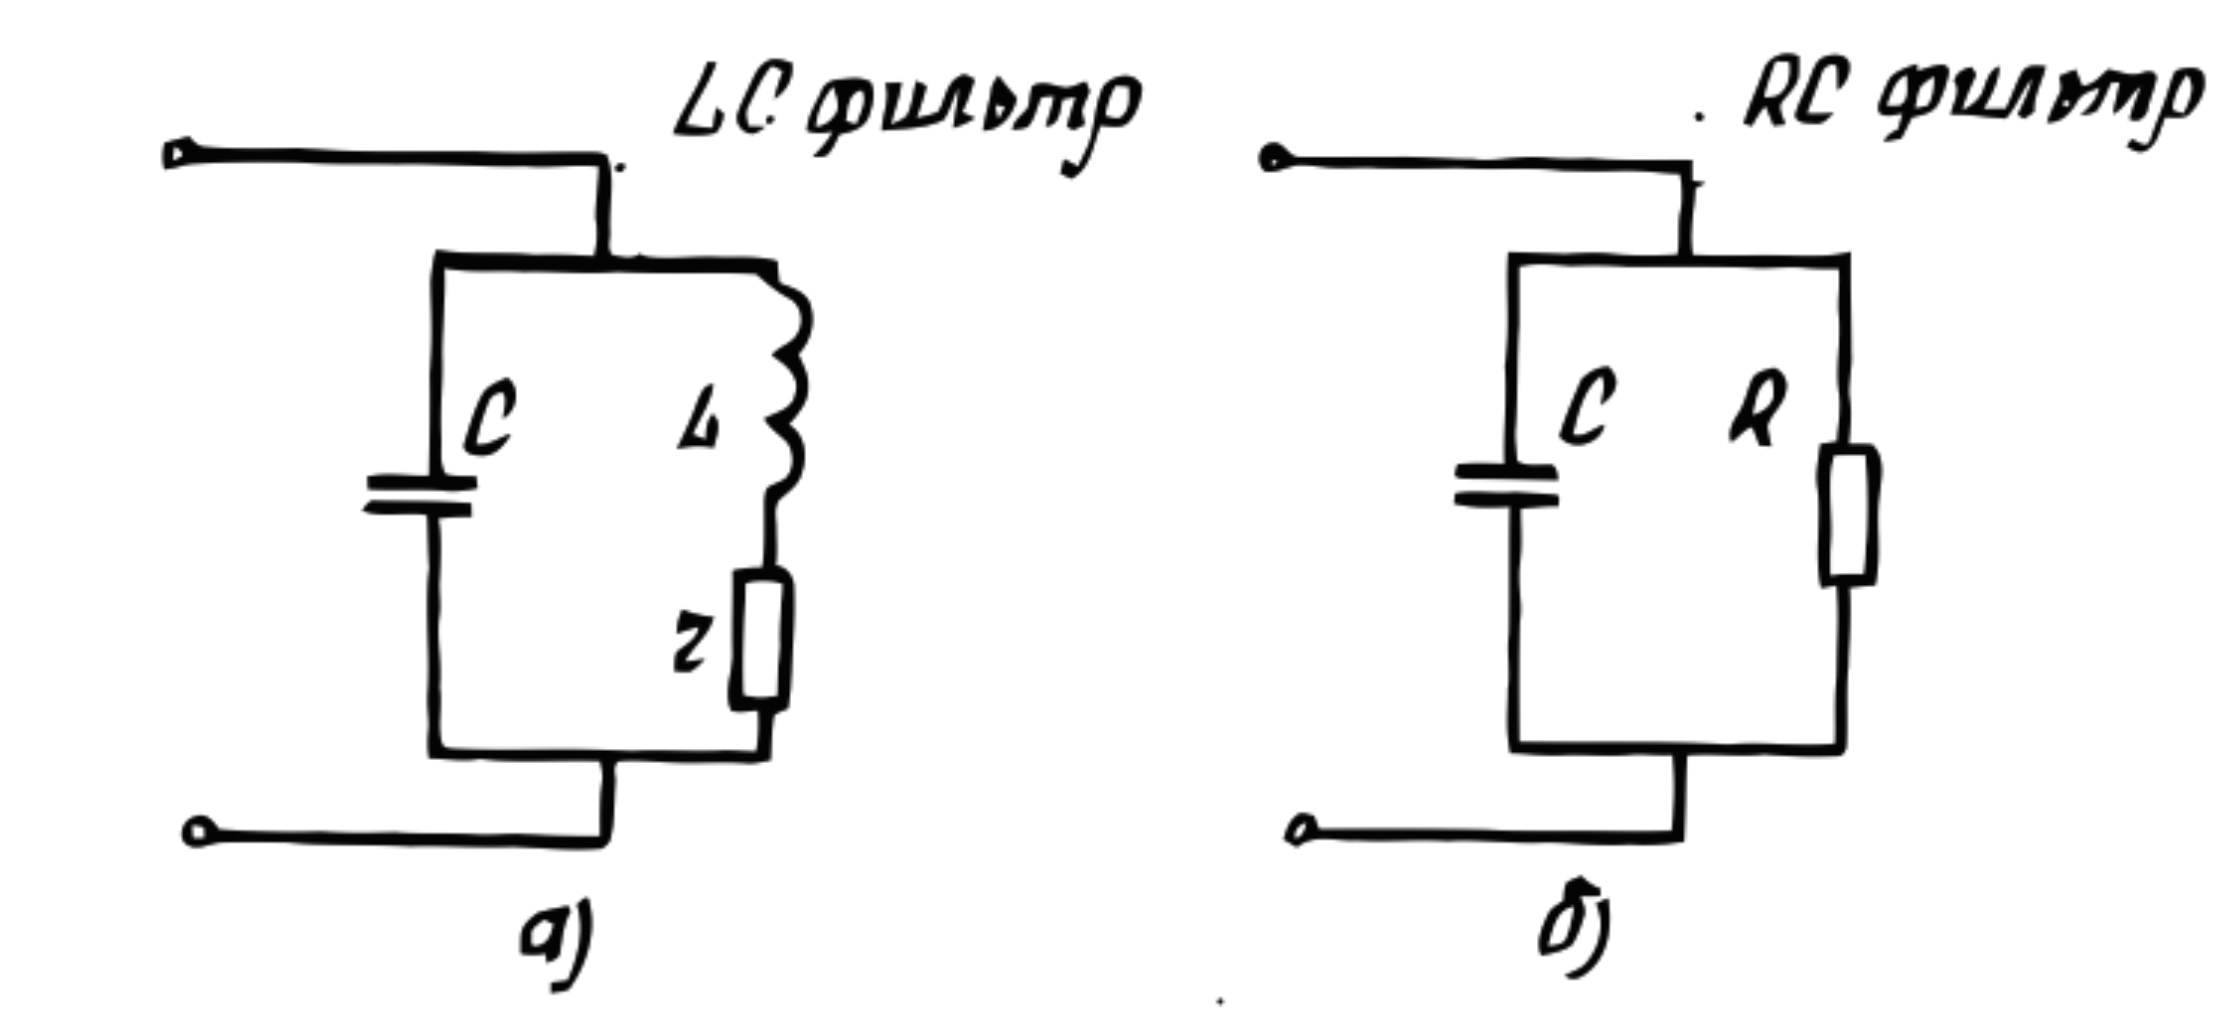
\includegraphics[width=0.5\textwidth]{picture/pic6.jpg}
		\vspace{-40pt}
	\end{center}
	\caption*{Рис. 1}
	\label{pic:6}
\end{wrapfigure}

Модуль импеданса параллельного контура (рис.~\ref{pic:6}а), настроенного на частоту $\omega_0$, определяется как
$$ Z=\frac{R_{\text{э}}}{\sqrt{1+Q^2\Delta^2}} $$
где $ R_{\text{э}} = \frac{L}{rC} $, $ Q = \frac{1}{r}\sqrt{\frac{C}{L}} $ , $ \Delta = \frac{\omega_0}{\omega}-\frac{\omega}{\omega_0} $ . На резонансной частоте $\omega_0$ сопротивление контура $Z = R_{\text{э}}$ наибольшее, с увеличением расстройки $Z$ убывает. Поэтому, когда через контур протекают различные компоненты тока, амплитуды которых одного порядка, значительное падение напряжения на нём создают только те компоненты, частоты которых близки к $\omega_0$. Компоненты тока с частотами, значительно отличающимися от
$\omega_0$, заметного напряжения не создают, благодаря чему в выходном напряжении они практически отсутствуют.

Модуль импеданса $Z$ цепочки $RC$ (рис.~\ref{pic:6}б)
$$ Z=\frac{R}{\sqrt{1+\omega^2R^2C^2}} $$
имеет максимальное значение $z = R$ при $\omega = 0$ и уменьшается с ростом частоты. Когда все составляющие тока протекают по такой цепи, заметное падение напряжения (выходное напряжение) создают только постоянная составляющая и составляющие низких частот. Скорость убывания $Z$ с частотой определяется выбором постоянной времени этой цепи, равной $\tau = RC$
\section{Преобразование частоты}
Сдвиг спектра сигнала по оси частот на определенную постоянную величину при сохранении структуры сигнала называется \textit{преобразованием частоты}.

Для выяснения процессов, происходящих при преобразовании частоты, вернемся к вопросу о воздействии на нелинейный элемент двух напряжений. Однако, в данном случае только одно из колебаний, колебание создаваемое вспомогательным генератором (гетеродином), будем считать гармоническим. Под вторым колебанием
будем подразумевать сигнал, подлежащий преобразованию, который может представлять собой любой сложный, но узкополосный процесс

Получаемое на выходе нелинейного элемента колебание с частотой $\omega_s(t)+\omega_{\text{г}}$ соответствует сдвигу спектра сигнала в область высоких частот, а колебание с частотой $\omega_s(t)+\omega_{\text{г}}$ в область низких частот. Для выделения одной из этих частот разностной или суммарной нужно применять соответствующую нагрузку на выходе преобразователя. Пусть, например, частоты $\omega_s$ и $\omega_{\text{г}}$ очень близки и требуется выделить низкую частоту, расположенную около нуля. Такая задача встречается в измерительной технике (метод "нулевых биений”). В этом случае нагрузка должна состоять из параллельного соединения $R$ и $С$ (рис.~\ref{pic:7}а), обеспечивающих отфильтровывание (подавление) высоких частот $\omega_s$ и $\omega_{\text{г}}$ и выделение разностной частоты $|\omega_s - \omega_{\text{г}}|$. Если частота	$|\omega_s - \omega_{\text{г}}|$ лежит в радиотехническом диапазоне, то для ее выделения следует применять колебательную цепь (рис.\ref{pic:7}б).
\begin{figure}[h!]
	\centering
	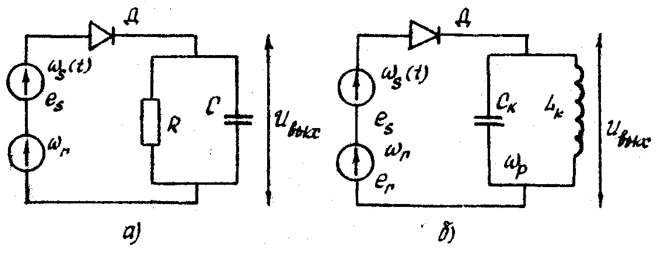
\includegraphics[width=0.7\textwidth]{picture/pic7.jpg}
	\caption{}
	\label{pic:7}
\end{figure}
\section{Амплитудное детектирование}
Детектированием принято называть преобразование модулированного колебания в
низкочастотное колебание, соответствующее модулирующему сигналу. Радиотехническое устройство, предназначенное для этой цели, называют детектором.

\begin{figure}[h!]
	\centering
	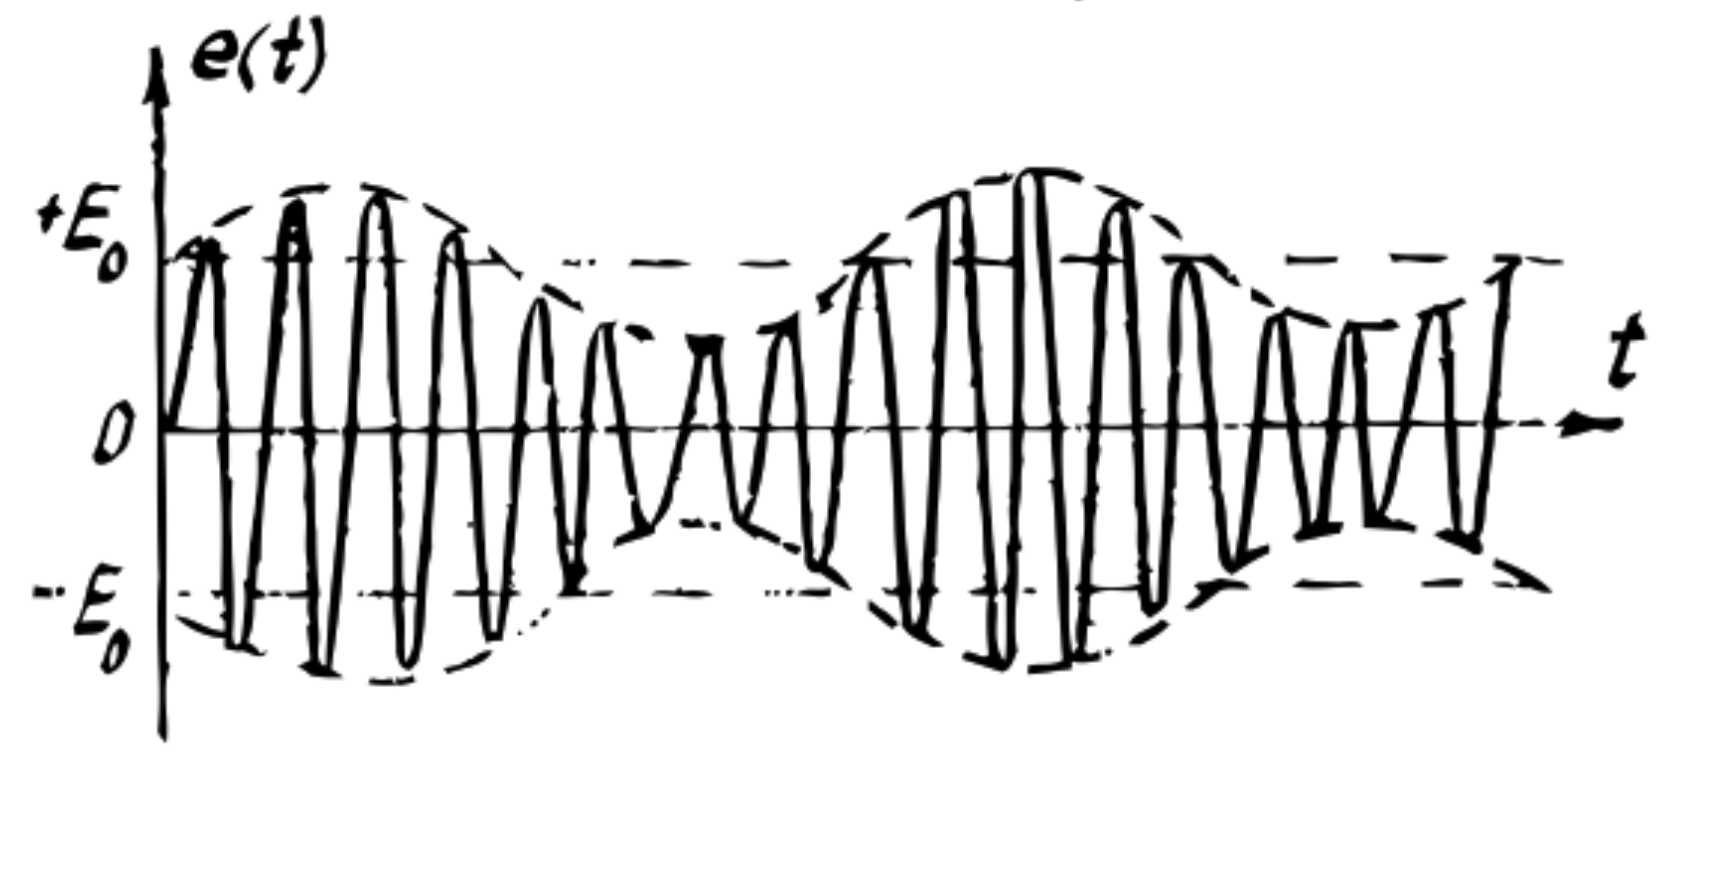
\includegraphics[width=0.7\textwidth]{picture/pic8.jpg}
	\caption{Амплитудно модулированное колебание}
	\label{pic:8}
\end{figure}

\begin{figure}[h!]
	\centering
	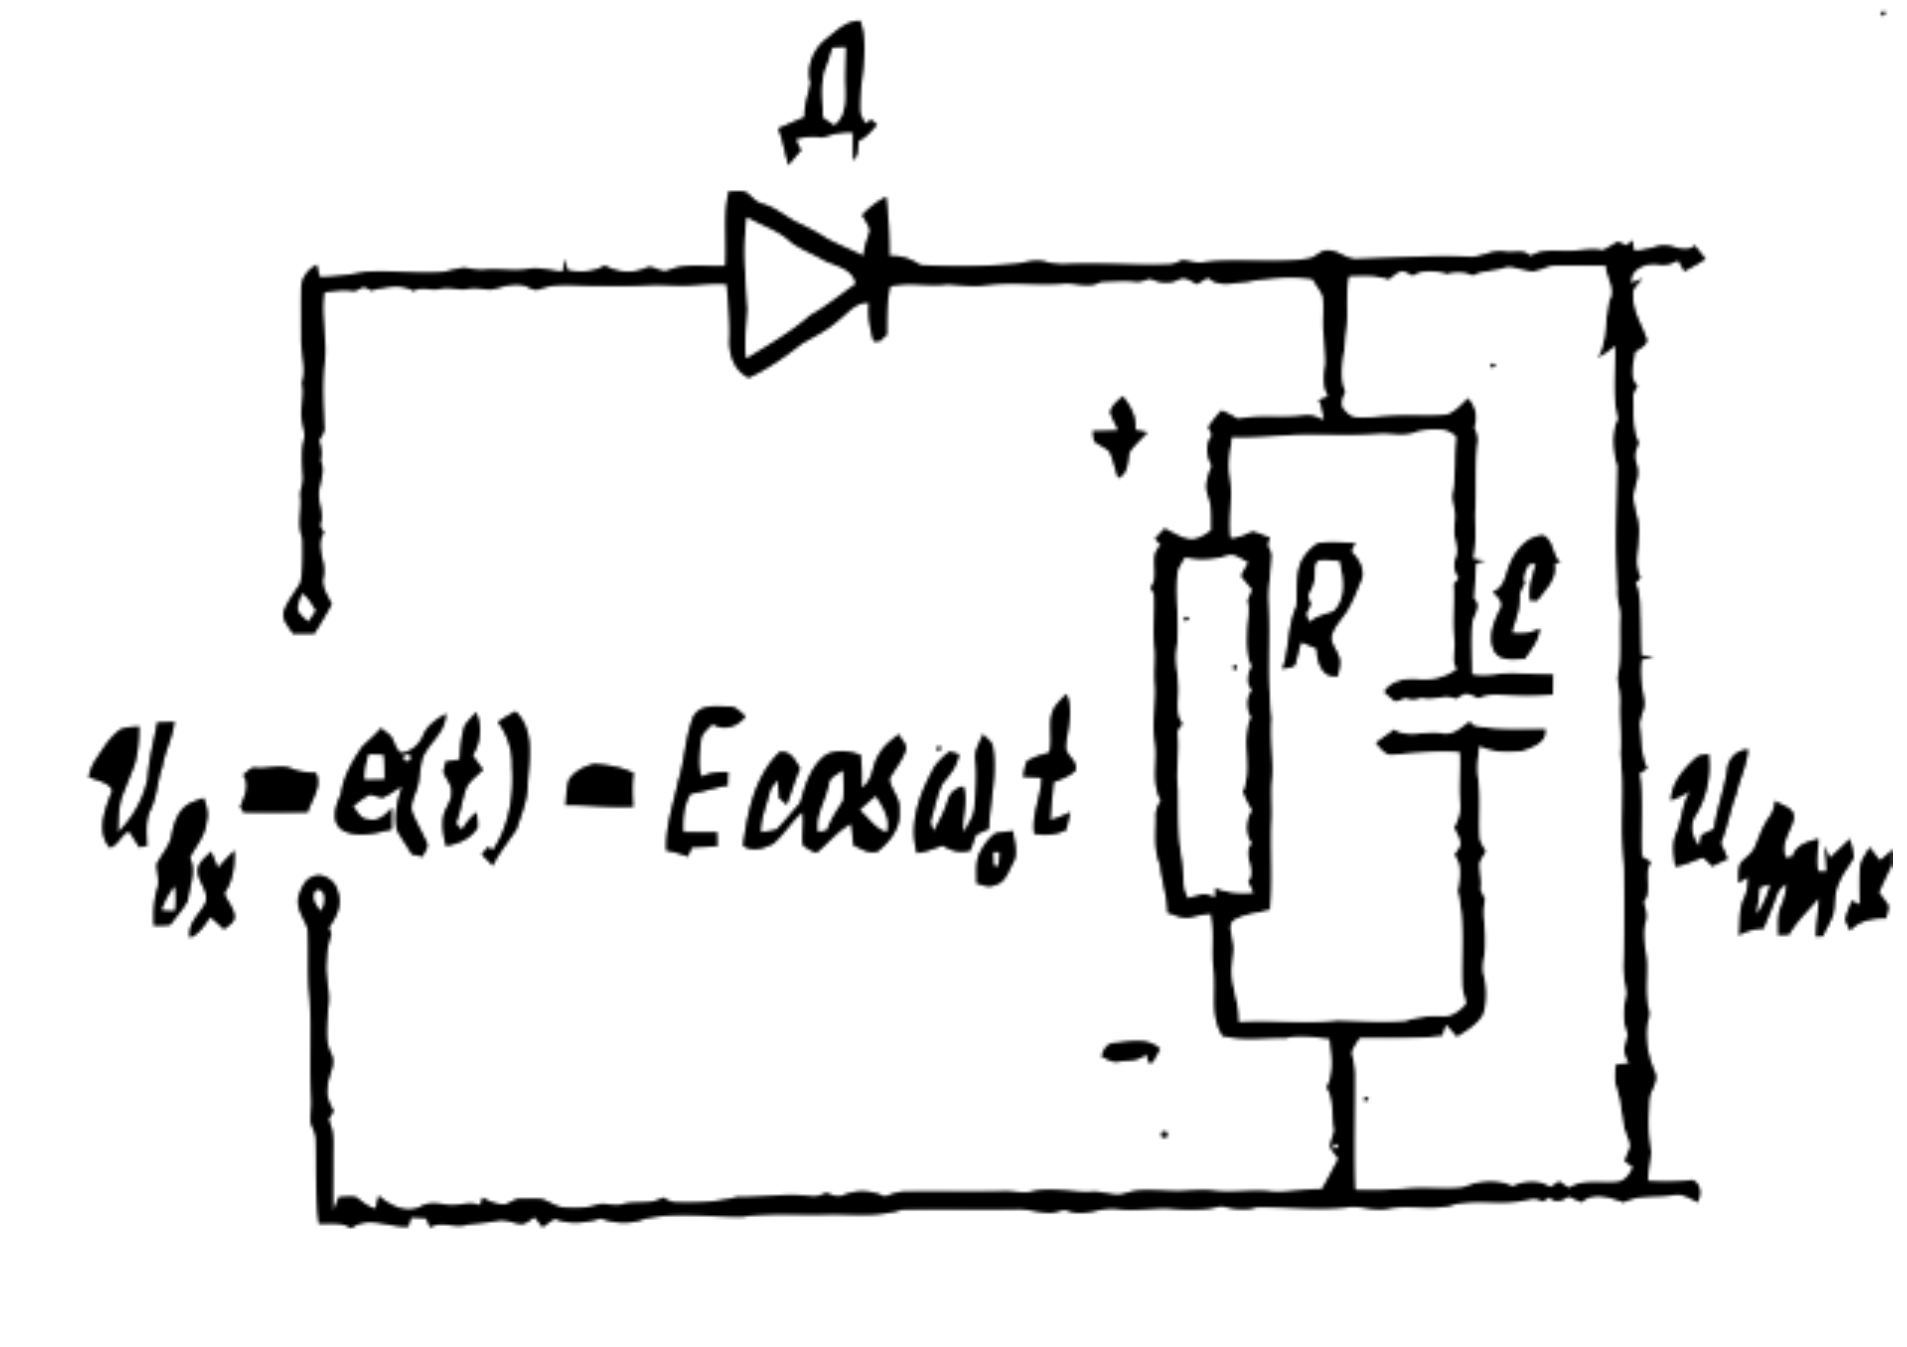
\includegraphics[width=0.6\textwidth]{picture/pic9.jpg}
	\caption{Амплитудный детектор}
	\label{pic:9}
\end{figure}
Рассмотрим высокочастотный сигнал, модулированный по амплитуде низкочастотным колебанием:
$$u(t)=E(1+M\cos{\Omega t})\cos{\omega_0 t},$$  $$\Omega \ll \omega_0 $$

$M$ - глубина модуляции. Пример такого колебания показан на рис.~\ref{pic:8}. В этом сигнале есть три гармоники: $ \omega_0 $, $ \omega_0 - \Omega$ и $\omega_0 + \Omega$. Подадим этот сигнал на диод. В выходном сигнале должен появиться набор комбинационных частот. Среди них будет гармоника с частотой $\Omega$. Частоты остальных гармоник будут много больше этой частоты. Для их устранения из выходного сигнала служит $RC$-фильтр. Таким образом, на выходе детектора получается колебание с частотой модуляции.

\begin{figure}[h!]
	\centering
	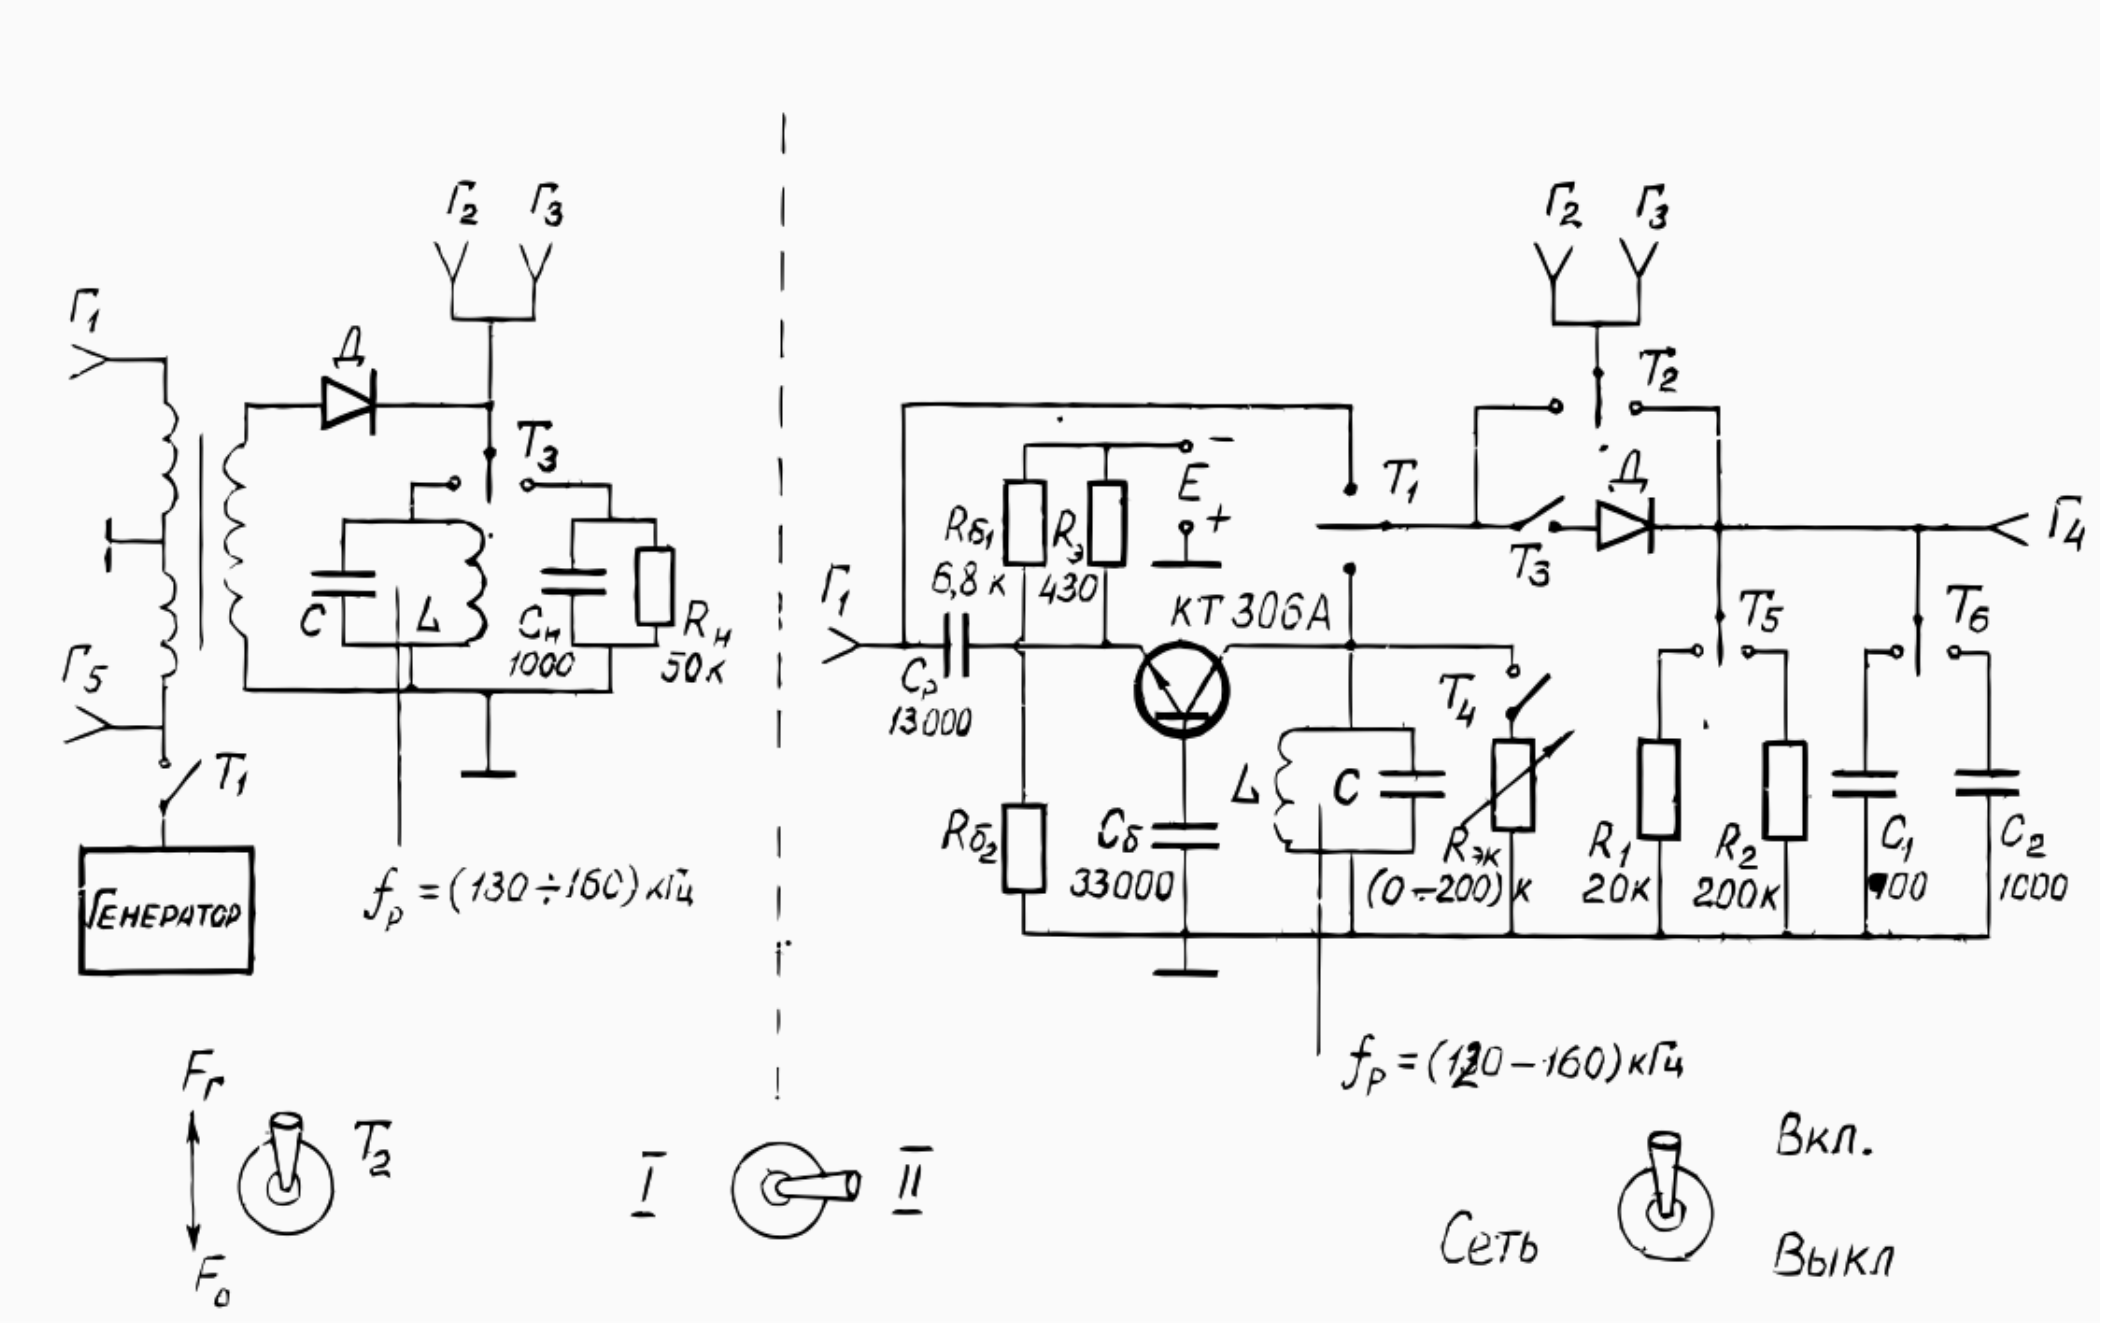
\includegraphics[width=\textwidth]{picture/pic10.jpg}
	\caption{Схема экспериментальной установки}
	\label{pic:10}
\end{figure}
\clearpage
\section[Задание 1]{Исследование нелинейности с апериодической нагрузкой}
Мы включили схему I (см. рис.~\ref{pic:10}). Тумблер $T_3$ поставили в положение $R_{\text{н}}$ н $C_{\text{н}}$,
тумблер $T_2$ - в положение $F_{\text{г}}$, тумблер $T_1$ - в положение “включено”(вверх). Затем мы
подключили генератор стандартных сигналов к гнезду $\Gamma_1$ и осциллограф к гнезду $\Gamma_3$.

Далее была снята зависимость выходного напряжения $U_{\text{вых}}$ на нагрузке $R_{\text{н}}$ от частоты $f_c$. 
\begin{figure}[h!]
	\centering
	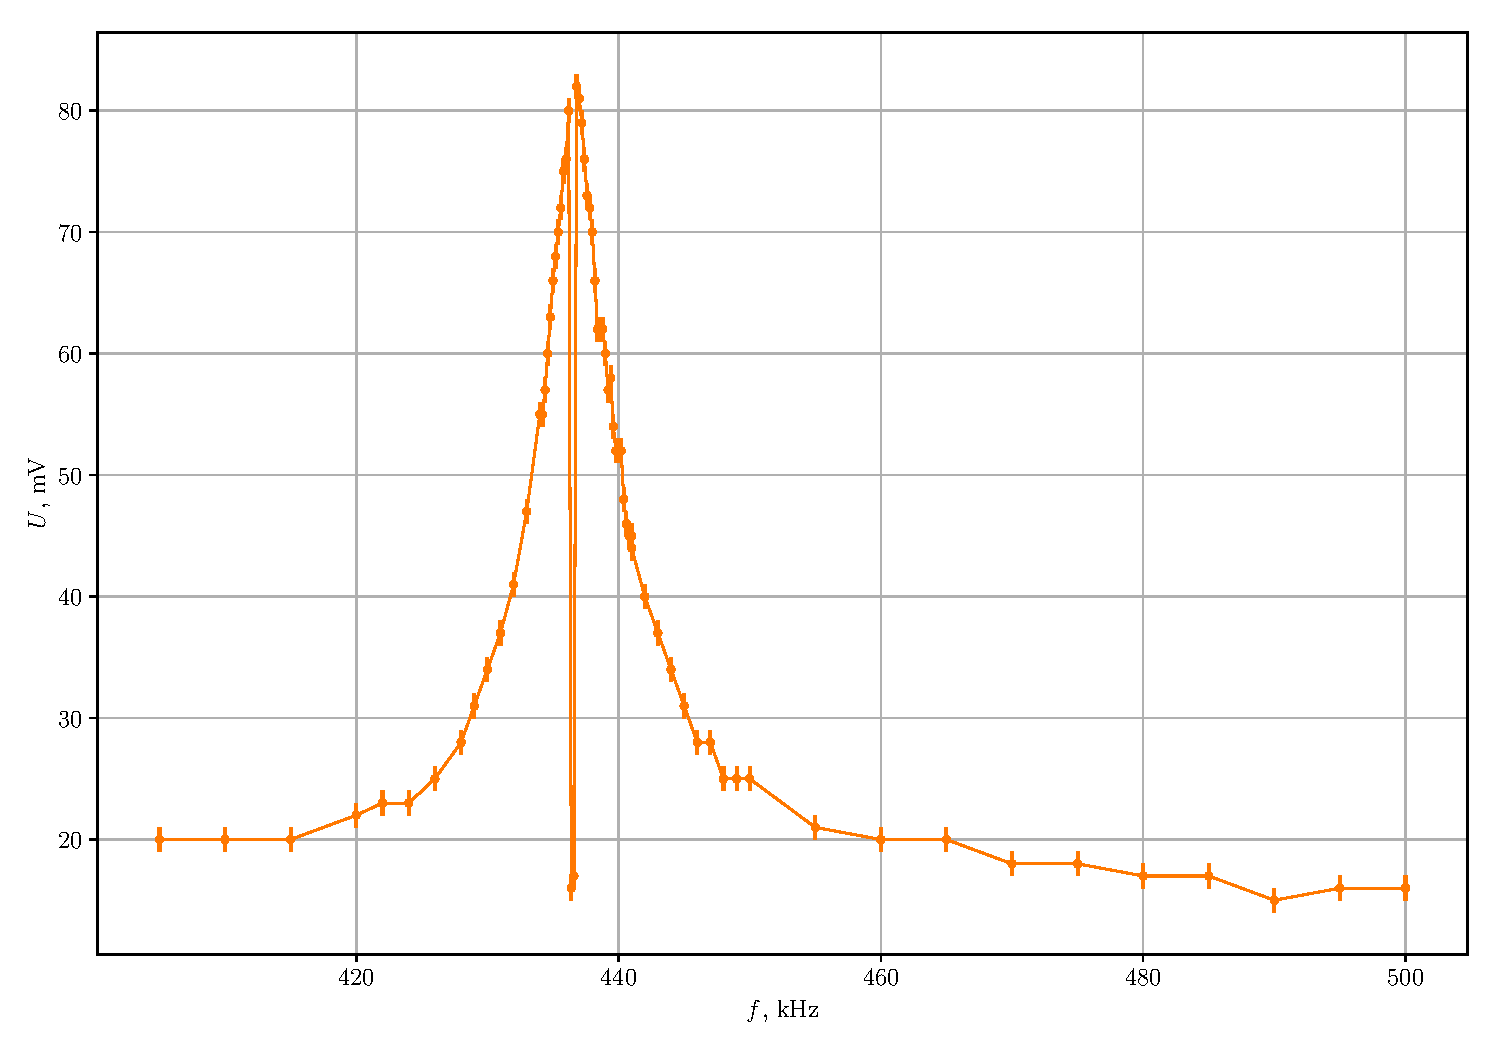
\includegraphics[width=\textwidth]{plots/exp1.pdf}
	\caption{выходное напряжение $U_{\text{вых}}$ на нагрузке $R_{\text{н}}$ от частоты $f_c$.}
	\label{exp:1}
\end{figure}

На графике $U_\text{вх}(f_c)$ заметен резкий спад амплитуды выходного сигнала на частоте нулевых биений $f_c=436.2\text{кГц}$. Метод нулевых биений -- это способ сравнения частот двух источников сигналов с целью подстройки одного источника под частоту другого, используя свойство колебаний с близкими, но не равными частотами, при наложении друг на друга создавать биения. В процессе подстройки частоту регулируемого источника изменяют таким образом, чтобы период биений увеличивался, до тех пор, пока биения не исчезнут, это будет означать, что частоты совпадают. 

Поскольку используются высокие частоты, суммарный сигнал подаётся на диодный детектор. Выделенные на диоде низкочастотные импульсы подаются на индикаторное устройство -- осциллограф.

Когда частота встроенного генератора совпала с частотой подаваемого сигнала огибающая стала содержать в себе только постоянную составляющую. Так как в настройках осциллографа использовали подавление постоянной составляющей сигнала, то на выходе наблюдали резкий спад амплитуды выходного сигнала. Таким образом определили частоту встроенного генератора $f_\text{г}=436.2\text{кГц}$.
\section[Задание 2]{Исследование нелинейности с резонансной нагрузкой}
Подключили осциллограф к гнезду $Г_3$ для измерения переменного напряжения,
тумблер $T_3$ перевели в положение “$LC$-контур”.
Была снята зависимость напряжения на контуре от частоты генератора стандартных сигналов $U_k=\phi(f_c)$.
\begin{figure}[h!]
	\centering
	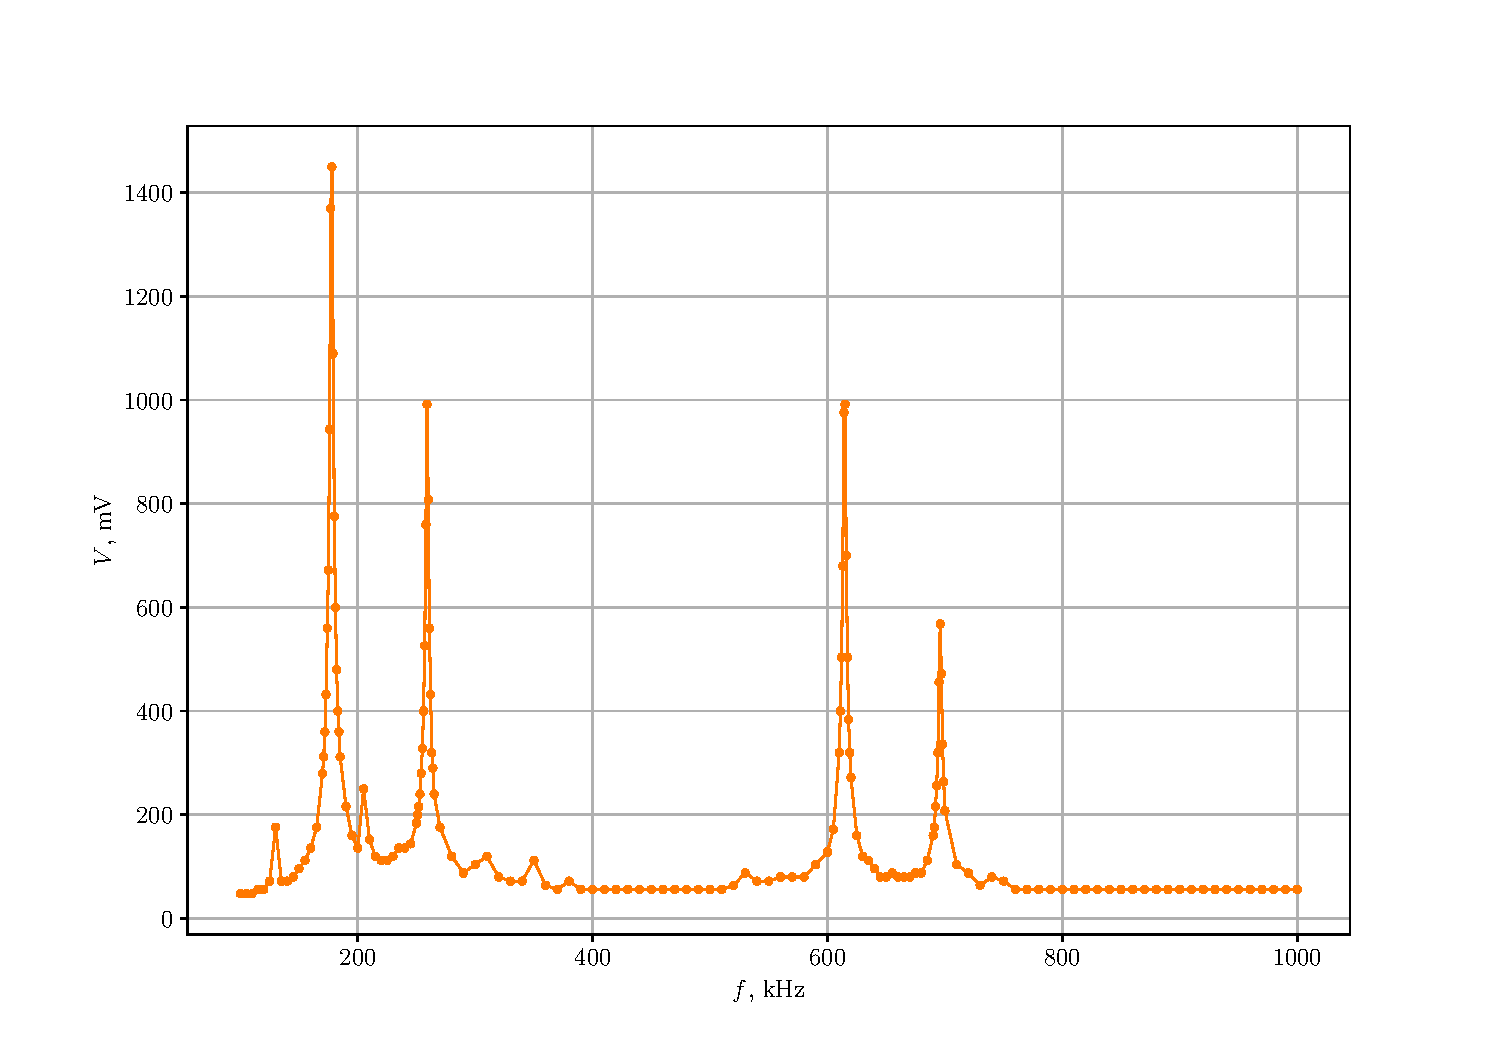
\includegraphics[width=\textwidth]{plots/exp2.pdf}
	\caption{напряжение на контуре от частоты генератора стандартных сигналов}
	\label{exp:2}
\end{figure}

В выходном сигнале нелинейной цепи должны присутствовать кратные и комбинационные частоты. Снятая зависимость представляет собой частотную характеристику преобразователя (зависимость модуля его комплексного коэффициента передачи от частоты принимаемого сигнала при постоянной частоте гетеродина). При взаимодействии колебаний некоторых
частот сигнала с колебаниями частот $\omega_{\text{г}}$ и $n\omega_{\text{г}}$ получаются колебания промежуточной
$\omega_{\text{пч}}$ частоты ($\omega_{\text{рез}} = \omega_{\text{пч}}$). Где $\omega_{\text{рез}}$ -- резонансная частота контура. Комбинационные частоты, совпадающие с $\omega_{\text{пч}}$, определяем в
виде $m\omega_{\text{г}} - n\omega_s = \omega_{\text{пч}}, m\omega_s - n\omega_{\text{г}} = \omega_{\text{пч}}$ откуда $\omega_s =\frac{n}{m}\omega_{\text{г}}\pm\frac{\omega_{\text{пч}}}{m}$.

При $n = 0$ и $m = 1$ частота $\omega_s$ соответствует частоте прямого канала, т.е. $\omega_s$ = $\omega _{\text{пч}}$.

При $n = 1$ и $m = 1$ преобразование осуществляется по первой гармонике частоты гетеродина: $\omega_{s} = \omega_{г} \pm \omega_{\text{пч}}$.

Из частотной характеристики преобразователя видно, что частоты каналов попарно
и симметрично расположены относительно частоты гетеродина и её гармоник, за исключением частоты прямого канала, равной $\omega_{\text{пч}}$. 
В нашем случае, резонансная частота колебательного контура $f_{\text{рез}} = f_{\text{пч}} = 178 \text{кГц}$.
$f_{\text{г}} - f_{\text{пч}} = 259 \text{кГц}$; $f_{\text{г}} + f_{\text{пч}} =615 \text{кГц}$. Тогда частота генератора $f_{\text{г}}= 437 \text{кГц}$. Сравнивая частоту генератора, найденную с помощью метода нулевых биений $f_{\text{г}}=436,2 \text{кГц}$, видим очень хорошее совпадение частот.
На графике $U_k(f_c)$ можно заметить еще один пик на частоте $f=696\text{кГц}$. Она возникает в следствие того, что нужно учитывать нелинейности более высокого порядка. Если мы будем аппроксимировать характеристику диода полиномом 3 степени, то в спектре должны появиться частоты $2f{\text{г}}-f_c=696 \text{кГц}$ и $f{\text{г}}-2f_c=81 \text{кГц}$, одна из которых видна на графике \ref{pic:10}.
\section[Задание 3]{Исследование амплитудного детектора}
Включив схему II, к гнезду $\text{Г}_3$ подключили осциллограф. Тумблером $T_1$ подключили детектор к гнезду $\text{Г}_1$, тумблер $T_5$ -- в положение $R_2$, тумблер $T_6$ -- в положение $C_2$, тумблер $T_3$ -- в положение “включено”. Затем мы подали на детектор сигнал с напряжением $U_{\text{вх}} = 1 \text{В}$ и частотой $f_c = 140 \text{кГц}$.
\subsection{Осциллограмма напряжения на входе и выходе детектора}
\begin{figure}[h!]
	\begin{minipage}{0.49\linewidth}
		\centering
		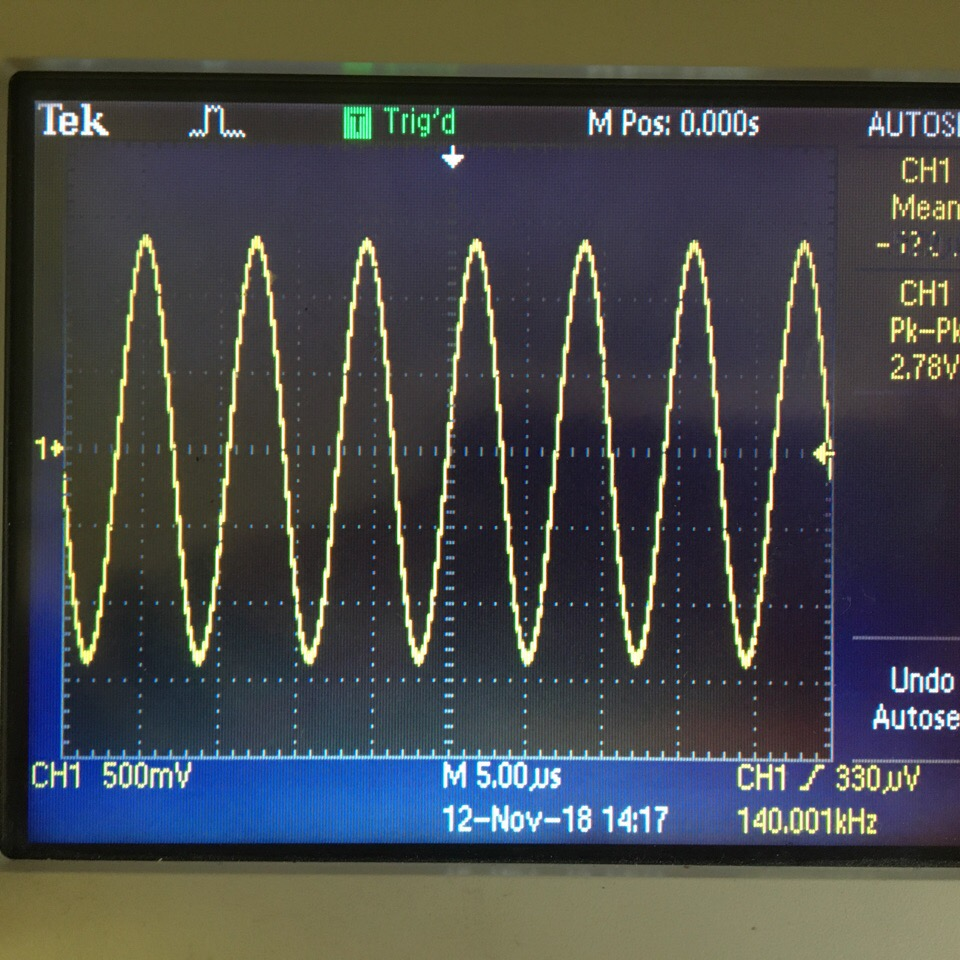
\includegraphics[width=0.8\linewidth]{photo/311.jpg}
		\caption{}
		\label{photo:3.1.1}
	\end{minipage}
	\begin{minipage}{0.49\linewidth}
		\centering
		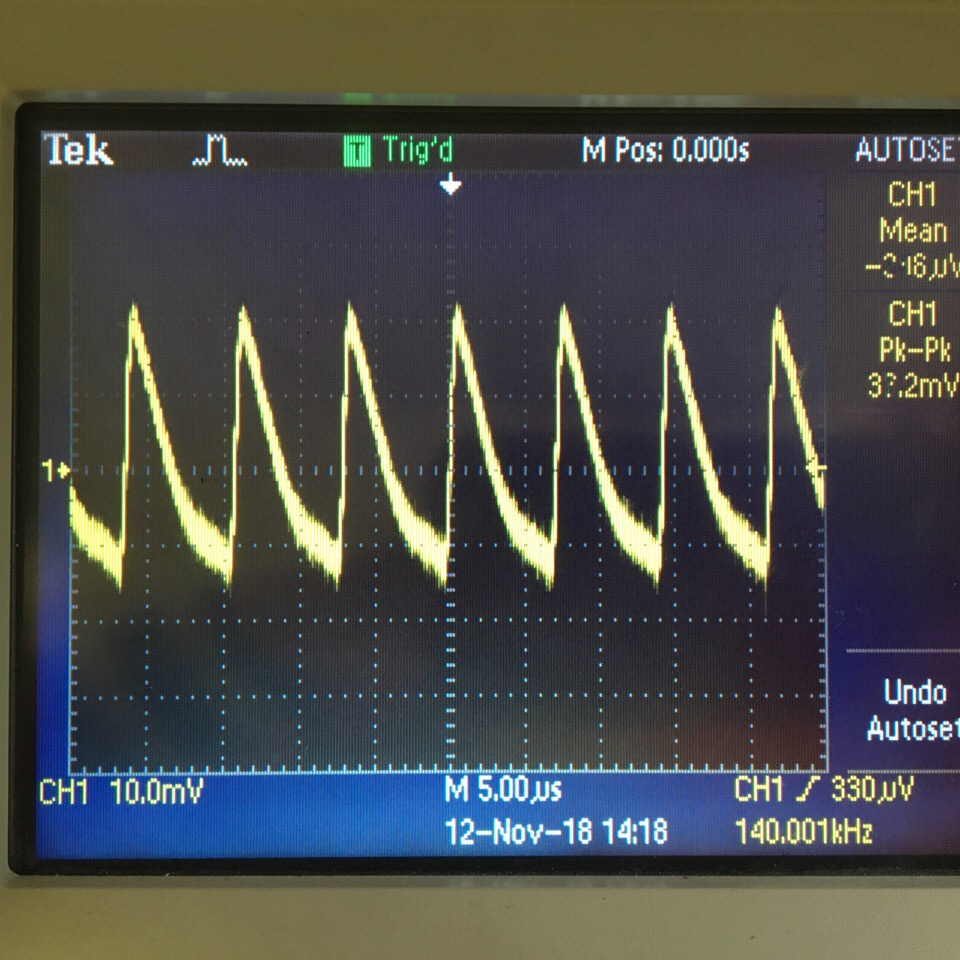
\includegraphics[width=0.8\linewidth]{photo/312.jpg}
		\caption{}
		\label{photo:3.1.2}
	\end{minipage}
\end{figure}
Напряжение на выходе детектора $u_\text{вых}(t)$ представляет собой колеблющуюся около среднего значения кривую. Это напряжение является напряжением смещения для диода. Поэтому ток через диод возможен только в течение отрезков периода, когда положительная полуволна ЭДС превышает напряжение $u_\text{вых}(t)$. Иными словами, ток через диод имеет форму импульсов. В промежутках между импульсами тока происходит разряд конденсатора $C$ через резистор $R$, и $u_\text{вых}(t)$ убывает.
\subsection{Зависимость выходного напряжения от амплитуды входного напряжения $u_\text{вых}=f(u_\text{вх})$}
\begin{figure}[h!]
	\centering
	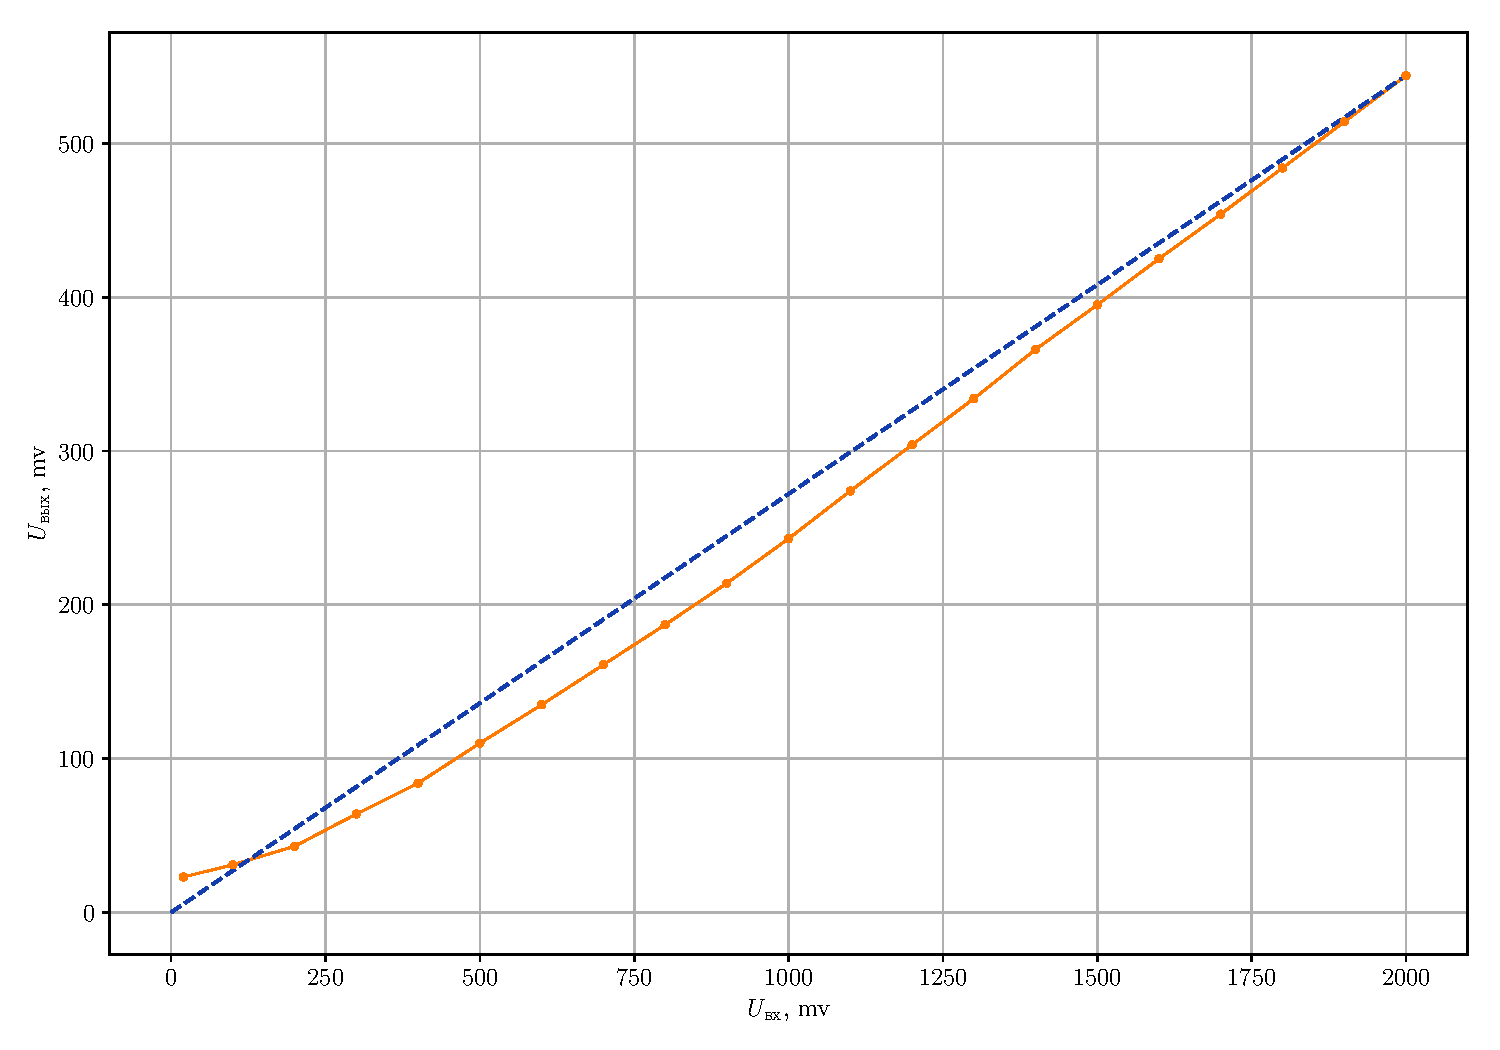
\includegraphics[width=0.8\linewidth]{plots/exp3a.pdf}
	\caption{}
	\label{exp:3.2}
\end{figure}

Когда режим работы детектора ничем не отличается от выпрямления высокочастотного сигнала с постоянной амплитудой $u_\text{вх}$, соотношение между $u_\text{вых}$ и $u_\text{вх}$ определяется выражением $u_\text{вых}=u_\text{вх}\cos\theta=const$, а так как угол отсечки $\theta$ мал, то отношение $u_\text{вых}/u_\text{вх}$ близко к 1.

Когда амплитуда $u_\text{вх}$ убывает почти до нуля выпрямление происходит на нижнем сгибе вольт-амперной характеристики. На этом участке детектирование является квадратичным. В результате характеристика детектирования принимает вид, представленный на графике ~\ref{exp:3.2}. При малых амплитудах она квадратична, при больших линейна.  
\subsection{Зависимость выходного напряжения от частоты модуляции  $u_{\text{вых}} = \phi(F_{\text{M}})$}
\begin{figure}
	\centering
	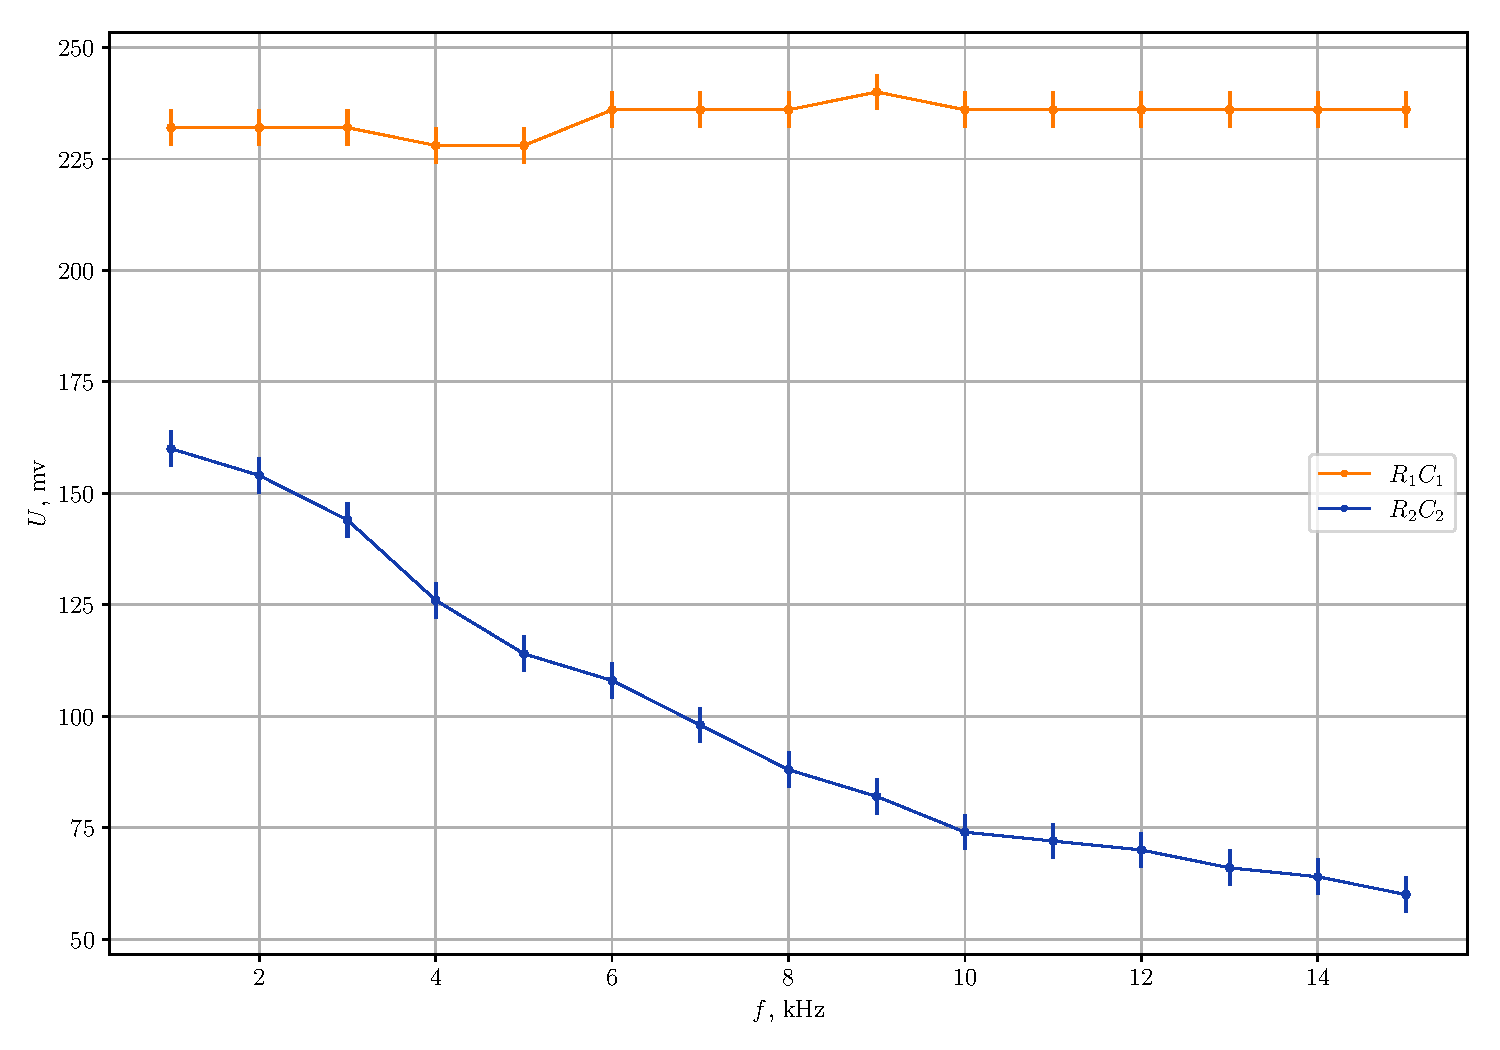
\includegraphics[width=0.8\linewidth]{plots/exp3b.pdf}
	\caption{}
	\label{exp:3.3}
\end{figure}
При выборе элементов нагрузки детектора необходимо, чтобы постоянная времени $RC$ была мала по сравнению с периодом модуляции. В противном случае изменение выпрямленного напряжения на нагрузке может отставать от изменения огибающей входной ЭДС Рис.~\ref{pic:11}. Получается нелинейное искажение сигнала. 
\begin{figure}[h!]
	\centering
	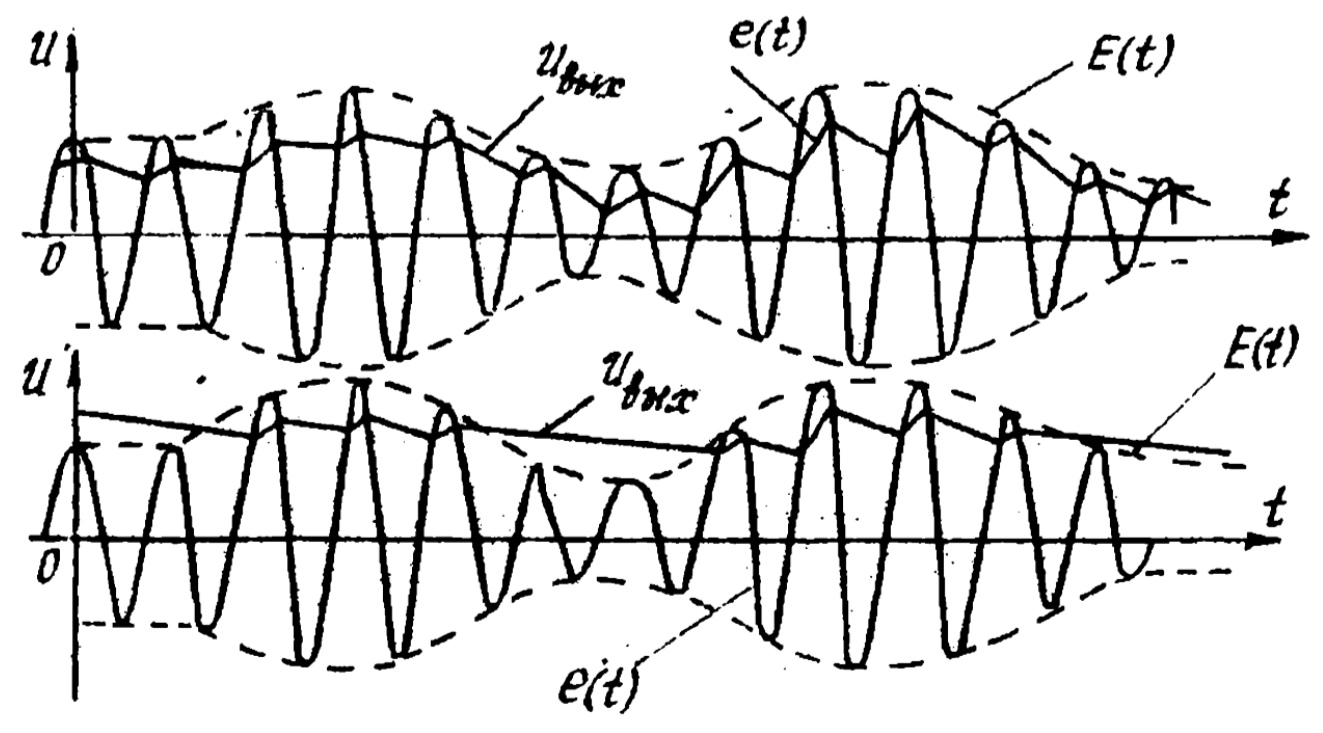
\includegraphics[width=0.8\linewidth]{picture/pic11.jpg}
	\caption{}
	\label{pic:11}
\end{figure}
Эти искажения обусловлены взаимодействием нелинейного элемента (диода) с линейной цепью $RC$, степень нелинейных искажений зависит не только от параметров цепи и глубины модуляции, но также от частоты модуляции. Эти искажения возрастают с повышением частоты, а также глубины модуляции входной ЭДС. Для устранения искажений необходимо $RC\ll2\pi/\Omega$. C другой стороны для сглаживания высокочастотных пульсаций необходимо, чтобы $RC\gg2\pi/\omega_c$. Совмещая эти условия получаем неравенство для выбора постоянно времени $RC$
$$\frac{2\pi}{\omega_c}\ll RC\ll\frac{2\pi}{\Omega}$$
В этой цепочки постоянные времени $R_1C_1=2\text{мс}$, $R_2C_2=200\text{мс}$. Сравнивая эти значения с характерным периодом модуляции сигнала (при $f_c=10\text{кГц}$ период модуляции равен $T_c=100\text{мс}$), заметим, что $R_2C_2>T_c$, что не удовлетворяет неравенству написанному выше. Таким образом зависимость $u_{\text{вых}} = \phi(F_\text{M})$ для цепочки $R_2C_2$ не является линейной.
\begin{figure}[h!]
	\begin{minipage}{0.33\linewidth}
		\centering
		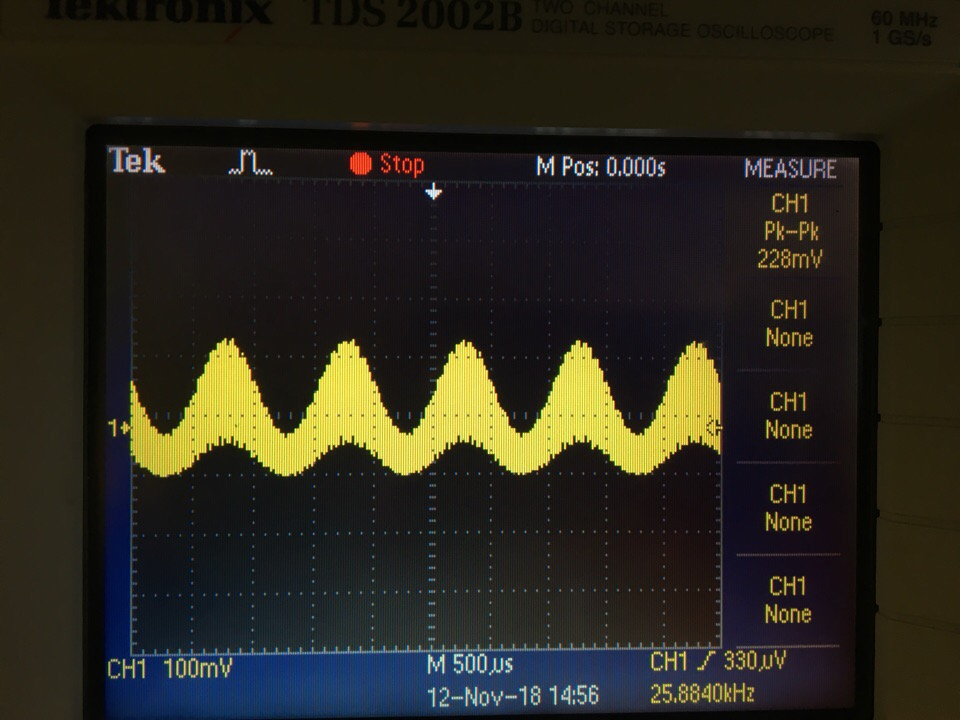
\includegraphics[width=0.9\linewidth]{photo/1kHztau1.jpg}
		\caption*{$R_1C_1$}
	\end{minipage}
	\begin{minipage}{0.33\linewidth}
		\centering
		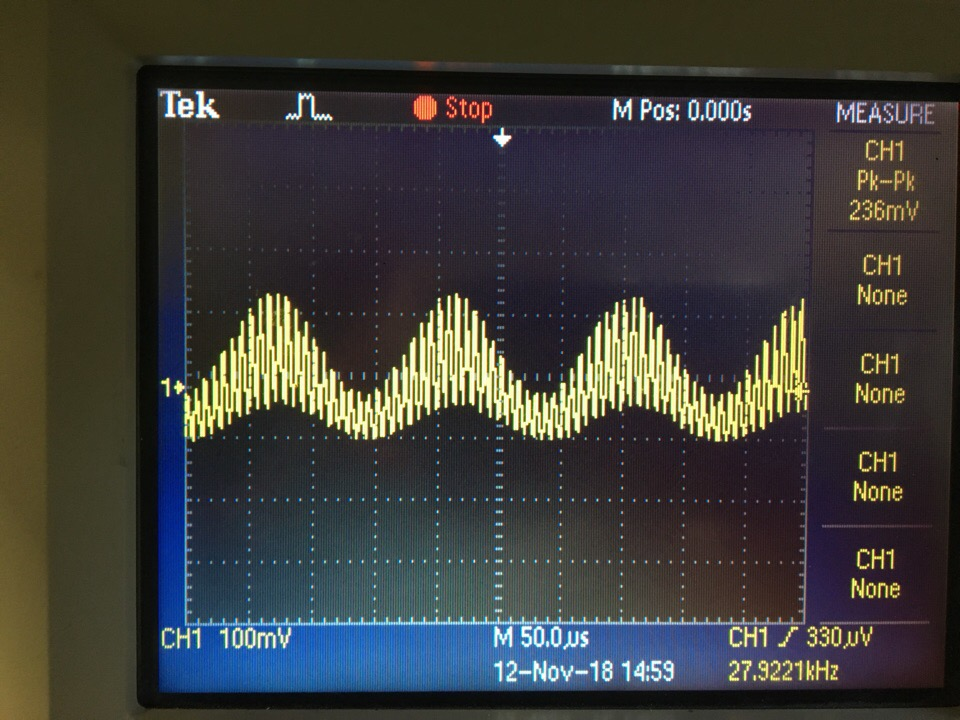
\includegraphics[width=0.9\linewidth]{photo/7kHztau1.jpg}
		\caption*{$R_1C_1$}
	\end{minipage}
	\begin{minipage}{0.33\linewidth}
		\centering
		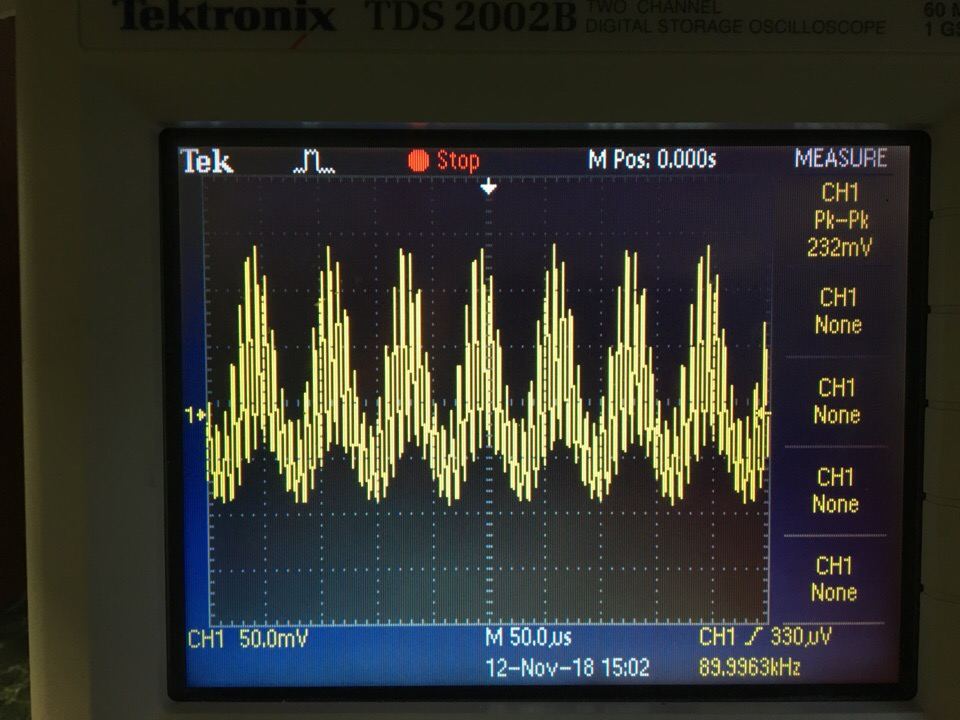
\includegraphics[width=0.9\linewidth]{photo/15kHztau1.jpg}
		\caption*{$R_1C_1$}
	\end{minipage}
	\begin{minipage}{0.33\linewidth}
		\centering
		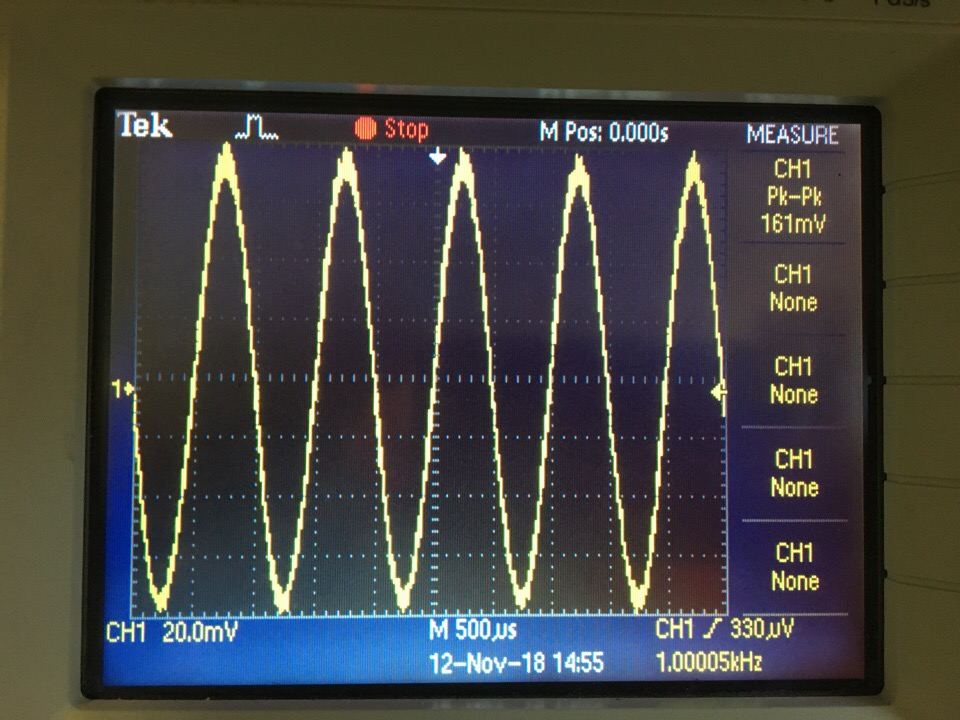
\includegraphics[width=0.9\linewidth]{photo/1kHztau2.jpg}
		\caption*{$R_2C_2$}
		\caption*{$F_\text{M}=1\text{кГц}$}
	\end{minipage}
	\begin{minipage}{0.33\linewidth}
		\centering
		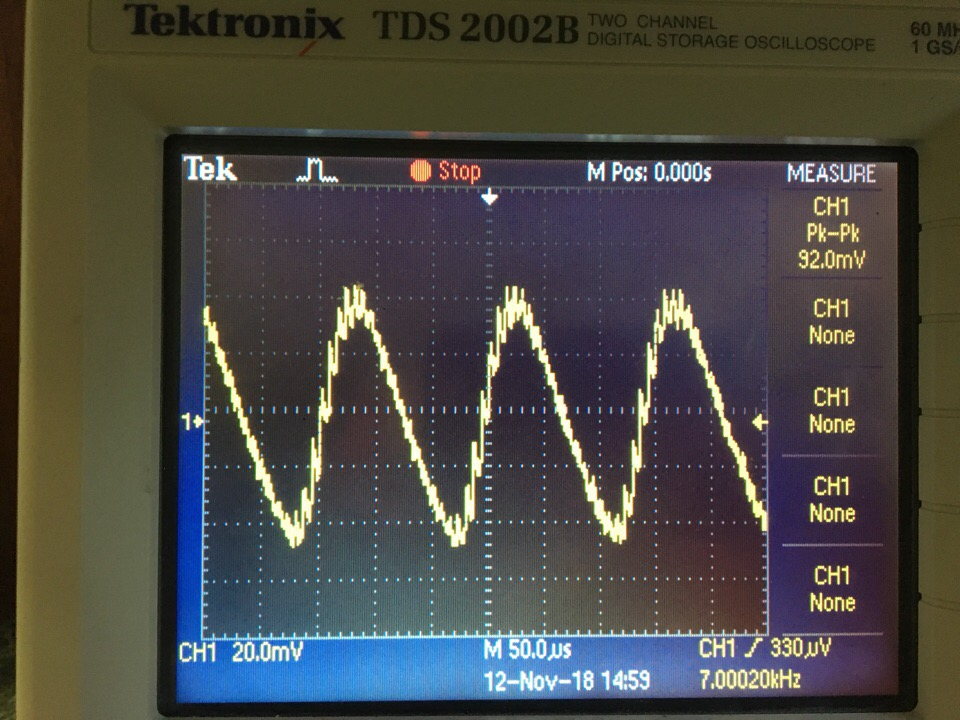
\includegraphics[width=0.9\linewidth]{photo/7kHztau2.jpg}
		\caption*{$R_2C_2$}
		\caption*{$F_\text{M}=7\text{кГц}$}
	\end{minipage}
	\begin{minipage}{0.33\linewidth}
		\centering
		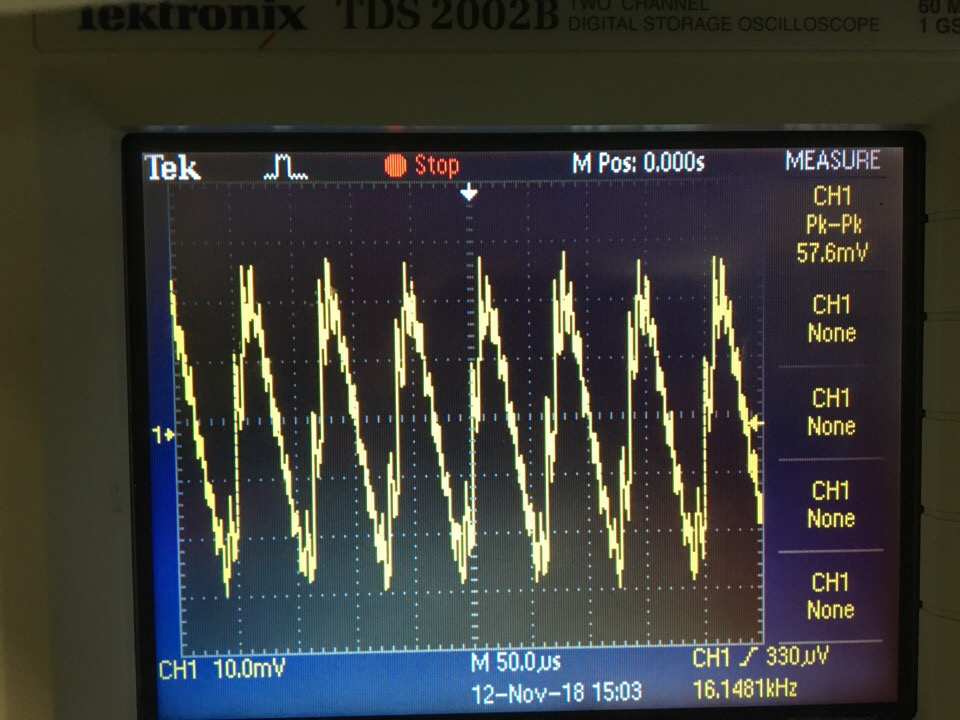
\includegraphics[width=0.9\linewidth]{photo/15kHztau2.jpg}
		\caption*{$R_2C_2$}
		\caption*{$F_\text{M}=15\text{кГц}$}
	\end{minipage}
\end{figure}
\subsection{Резонансные характеристики усилителя}
 \begin{figure}[h!]
	\centering
	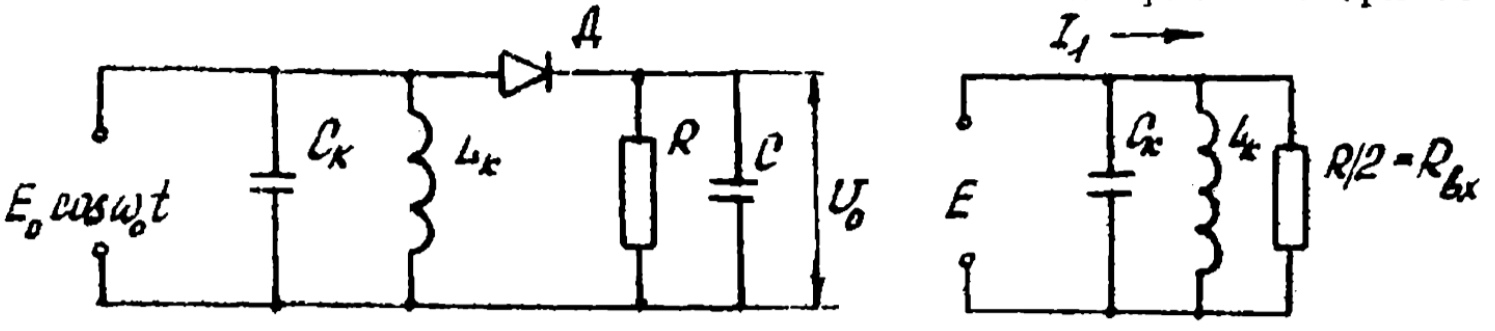
\includegraphics[width=\linewidth]{picture/pic12.jpg}
	\caption{}
	\label{pic:12}
\end{figure}

 \begin{figure}[H]
 	\centering
 	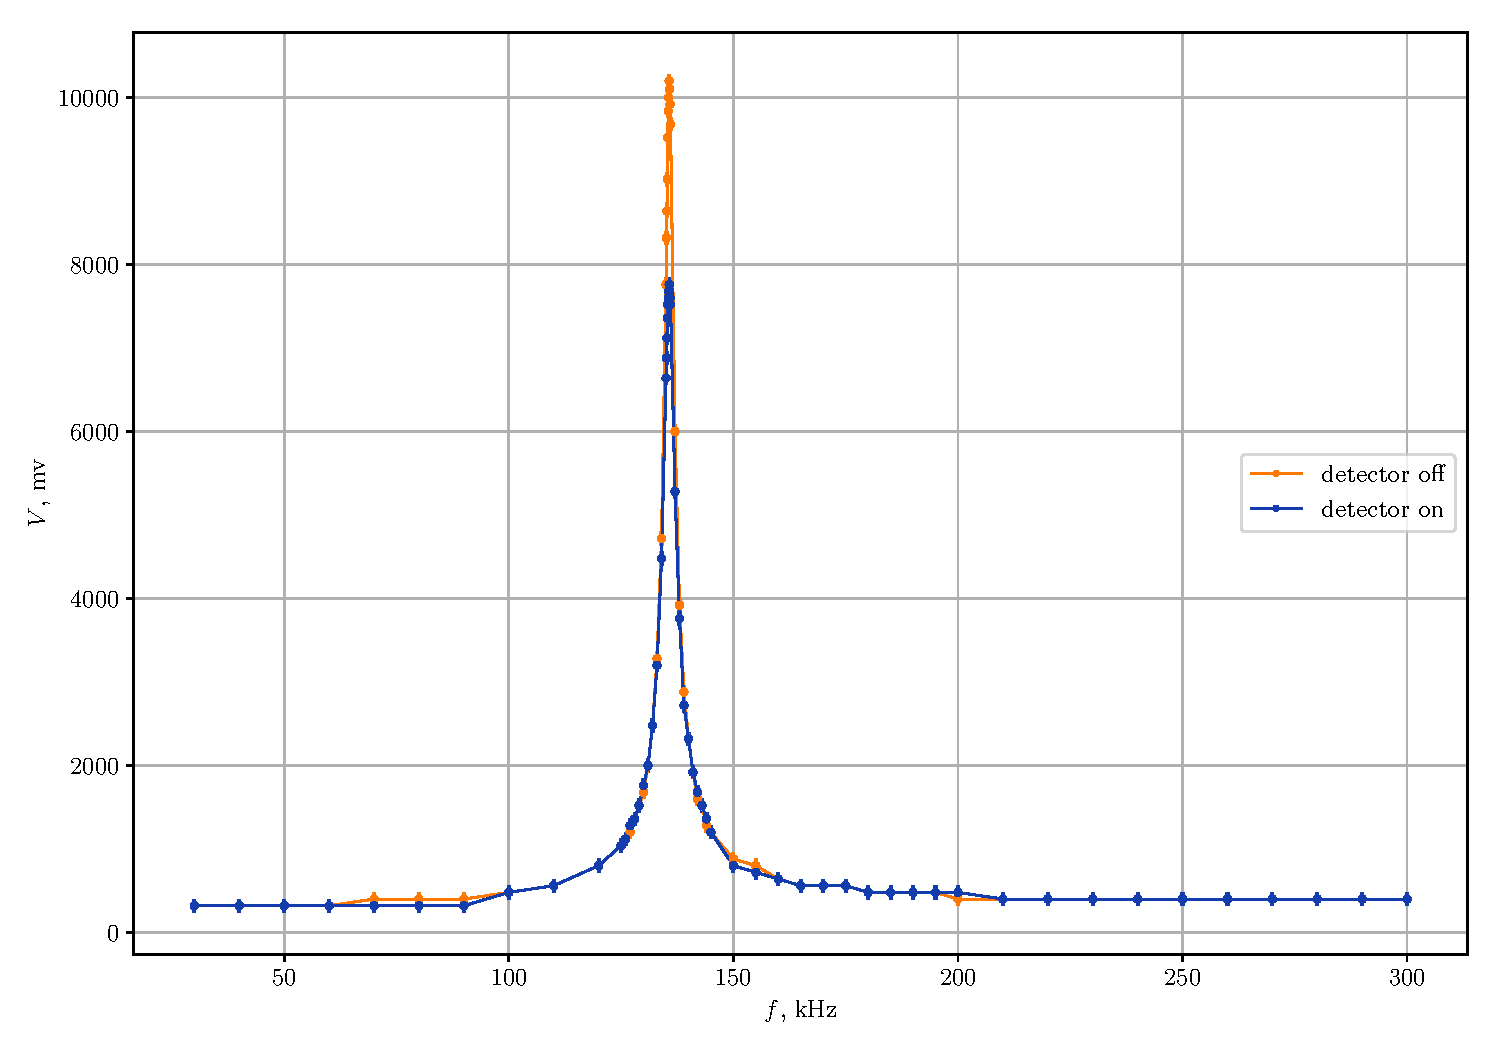
\includegraphics[width=\linewidth]{plots/exp3c.pdf}
 	\caption{}
 	\label{exp:3.4}
 \end{figure}
\subsection{Входное сопротивление детектора}
На вход усилителя был подан немодулированный сигнал от генератора стандартных
сигналов с напряжением $u_{\text{вх}} = 1\text{В}$ и установлена нагрузка $R_2 C_2$. Сопротивление $R_{\text{экв}}$  отключено. Зафиксировали максимальное значение на контуре при подключенном детекторе. Отключили детектор и подключили $R_{\text{экв}}$. Изменяя $R_{\text{экв}}$,достигли того, что напряжение на контуре стало равно максимальному значению при подключенном детекторе. Соответствующее этому значению $R_{\text{экв}} =99 \text{кОм}$. $R_{\text{вх}} = 2R_{\text{экв}} = 198\text{кОм}$. 
\section{Вывод}
Изучили основные процессы, происходящие при прохождении сигналов через радиотехнических цепи с нелинейными элементами, эксперементально исследовали характеристики полупроводникового преобразователя частоты и амплитудного диодного детектора. 
\end{document}
